\INEchaptercarta[Gasto público y financiamiento]{Gasto público y\\ financiamiento}{}


\cajita{Evolución del gasto, por sector}{El gasto público en educación en el 2013 fue de Q12,896, del cual el 83.3\% se destinó a entidades centralizadas. En el 2012 fue asignado a este sector el 83.6\%.\\
	
	\textollamada[*]{ Dentro este tipo de entidades se encuentra: el Ministerio de Educación, Ministerio de la Defensa, Ministerio de Salud Pública y Asistencia Social y el Ministerio de Agricultura, Ganadería y Alimentación.}}{Gasto público en educación, por sector}{República de Guatemala, 2012 y 2013, en millones de quetzales de cada año}{
		\ra{1.2}$\ $\\
		\begin{tabular}{p{3.5cm}x{2cm}x{2cm}}\hline
		\rowcolor{color2!15!white} &&\\[-4mm]
		{\Bold    Sector          }&      \textbf{ 2012 }  &  \textbf{ 2013 }   \\
		\hline
		\rowcolor{white} &&\\[-4mm]
		
	\textbf{Total general} &	\textbf{12,133}& 	\textbf{12,896} \\
	Centralizadas&	10,147& 	10,749 \\
	Descentralizadas&	1,986 &	2,148 \\
		\hline
		&&\\[2mm]
		\end{tabular}
		}{Instituto Nacional de Estadística}


\cajita{Gasto por sector}{Según el sector de las entidades en educación, estas son centralizadas o descentralizadas. En el año 2013 el 16.7\% de los recursos del gasto público en educación fue asignado a las entidades descentralizadas.\\
	
	Entre las entidades descentralizadas se incluye: la Universidad de San Carlos de Guatemala, el Instituto Técnico de Capacitación y Productividad, el Comité Nacional de Alfabetización y la Escuela Nacional Central de Agricultura.}{Distribución de gasto público, por sector}{República de Guatemala, 2013, en porcentaje}{\ \\[0mm]\begin{tikzpicture}[x=1pt,y=1pt]  % Created by tikzDevice version 0.7.0 on 2015-08-28 13:12:34
% !TEX encoding = UTF-8 Unicode
\definecolor[named]{fillColor}{rgb}{1.00,1.00,1.00}
\path[use as bounding box,fill=fillColor,fill opacity=0.00] (0,0) rectangle (289.08,198.74);
\begin{scope}
\path[clip] ( 30.54,  0.00) rectangle (258.54,198.74);
\definecolor[named]{drawColor}{rgb}{1.00,1.00,1.00}

\path[draw=drawColor,line width= 0.6pt,line join=round,line cap=round] ( 30.54,  0.00) rectangle (258.54,198.74);
\end{scope}
\begin{scope}
\path[clip] (  0.00,  0.00) rectangle (289.08,198.74);

\path[] (  9.28,  7.11) rectangle (200.91,198.74);

\path[] (105.09,102.93) --
	(191.31,101.55);

\path[] (105.09,102.93) --
	( 18.87,104.30);

\path[] (105.09,102.93) --
	(106.47,189.15);

\path[] (105.09,102.93) --
	(191.31,101.55);

\path[] (105.09,102.93) --
	(103.72, 16.71);

\path[] (105.09,102.93) --
	( 18.87,104.30);

\path[] (105.09,102.93) --
	(105.09,102.93) --
	(105.09,102.93) --
	(105.09,102.93) --
	(105.09,102.93) --
	(105.09,102.93) --
	(105.09,102.93) --
	(105.09,102.93) --
	(105.09,102.93) --
	(105.09,102.93) --
	(105.09,102.93) --
	(105.09,102.93) --
	(105.09,102.93) --
	(105.09,102.93) --
	(105.09,102.93) --
	(105.09,102.93) --
	(105.09,102.93) --
	(105.09,102.93) --
	(105.09,102.93) --
	(105.09,102.93) --
	(105.09,102.93) --
	(105.09,102.93) --
	(105.09,102.93) --
	(105.09,102.93) --
	(105.09,102.93) --
	(105.09,102.93) --
	(105.09,102.93) --
	(105.09,102.93) --
	(105.09,102.93) --
	(105.09,102.93) --
	(105.09,102.93) --
	(105.09,102.93) --
	(105.09,102.93) --
	(105.09,102.93) --
	(105.09,102.93) --
	(105.09,102.93) --
	(105.09,102.93) --
	(105.09,102.93) --
	(105.09,102.93) --
	(105.09,102.93) --
	(105.09,102.93) --
	(105.09,102.93) --
	(105.09,102.93) --
	(105.09,102.93) --
	(105.09,102.93) --
	(105.09,102.93) --
	(105.09,102.93) --
	(105.09,102.93) --
	(105.09,102.93) --
	(105.09,102.93) --
	(105.09,102.93) --
	(105.09,102.93) --
	(105.09,102.93) --
	(105.09,102.93) --
	(105.09,102.93) --
	(105.09,102.93) --
	(105.09,102.93) --
	(105.09,102.93) --
	(105.09,102.93) --
	(105.09,102.93) --
	(105.09,102.93) --
	(105.09,102.93) --
	(105.09,102.93) --
	(105.09,102.93) --
	(105.09,102.93) --
	(105.09,102.93) --
	(105.09,102.93) --
	(105.09,102.93) --
	(105.09,102.93) --
	(105.09,102.93) --
	(105.09,102.93) --
	(105.09,102.93) --
	(105.09,102.93) --
	(105.09,102.93) --
	(105.09,102.93) --
	(105.09,102.93) --
	(105.09,102.93) --
	(105.09,102.93) --
	(105.09,102.93) --
	(105.09,102.93) --
	(105.09,102.93) --
	(105.09,102.93) --
	(105.09,102.93) --
	(105.09,102.93) --
	(105.09,102.93) --
	(105.09,102.93) --
	(105.09,102.93) --
	(105.09,102.93) --
	(105.09,102.93) --
	(105.09,102.93) --
	(105.09,102.93) --
	(105.09,102.93) --
	(105.09,102.93) --
	(105.09,102.93) --
	(105.09,102.93) --
	(105.09,102.93) --
	(105.09,102.93) --
	(105.09,102.93) --
	(105.09,102.93) --
	(105.09,102.93);

\path[] (105.09,122.09) --
	(106.31,122.05) --
	(107.52,121.94) --
	(108.72,121.74) --
	(109.90,121.48) --
	(111.07,121.13) --
	(112.21,120.72) --
	(113.33,120.23) --
	(114.41,119.67) --
	(115.45,119.05) --
	(116.45,118.36) --
	(117.41,117.61) --
	(118.32,116.80) --
	(119.17,115.93) --
	(119.96,115.01) --
	(120.70,114.04) --
	(121.37,113.03) --
	(121.98,111.98) --
	(122.52,110.89) --
	(122.99,109.77) --
	(123.39,108.62) --
	(123.71,107.45) --
	(123.96,106.26) --
	(124.14,105.05) --
	(124.23,103.84) --
	(124.25,102.62) --
	(124.19,101.41) --
	(124.06,100.20) --
	(123.85, 99.00) --
	(123.56, 97.82) --
	(123.20, 96.66) --
	(122.77, 95.52) --
	(122.26, 94.42) --
	(121.69, 93.35) --
	(121.05, 92.31) --
	(120.34, 91.32) --
	(119.57, 90.38) --
	(118.75, 89.49) --
	(117.87, 88.65) --
	(116.94, 87.86) --
	(115.96, 87.14) --
	(114.93, 86.49) --
	(113.87, 85.90) --
	(112.77, 85.37) --
	(111.65, 84.92) --
	(110.49, 84.54) --
	(109.31, 84.24) --
	(108.12, 84.01) --
	(106.91, 83.85) --
	(105.70, 83.77) --
	(104.48, 83.77) --
	(103.27, 83.85) --
	(102.06, 84.01) --
	(100.87, 84.24) --
	( 99.69, 84.54) --
	( 98.54, 84.92) --
	( 97.41, 85.37) --
	( 96.31, 85.90) --
	( 95.25, 86.49) --
	( 94.22, 87.14) --
	( 93.25, 87.86) --
	( 92.31, 88.65) --
	( 91.43, 89.49) --
	( 90.61, 90.38) --
	( 89.84, 91.32) --
	( 89.14, 92.31) --
	( 88.50, 93.35) --
	( 87.92, 94.42) --
	( 87.42, 95.52) --
	( 86.98, 96.66) --
	( 86.62, 97.82) --
	( 86.33, 99.00) --
	( 86.12,100.20) --
	( 85.99,101.41) --
	( 85.93,102.62) --
	( 85.95,103.84) --
	( 86.05,105.05) --
	( 86.22,106.26) --
	( 86.47,107.45) --
	( 86.79,108.62) --
	( 87.19,109.77) --
	( 87.66,110.89) --
	( 88.20,111.98) --
	( 88.81,113.03) --
	( 89.48,114.04) --
	( 90.22,115.01) --
	( 91.01,115.93) --
	( 91.87,116.80) --
	( 92.77,117.61) --
	( 93.73,118.36) --
	( 94.73,119.05) --
	( 95.77,119.67) --
	( 96.85,120.23) --
	( 97.97,120.72) --
	( 99.11,121.13) --
	(100.28,121.48) --
	(101.46,121.74) --
	(102.67,121.94) --
	(103.88,122.05) --
	(105.09,122.09);

\path[] (105.09,141.25) --
	(107.52,141.18) --
	(109.94,140.95) --
	(112.34,140.56) --
	(114.72,140.03) --
	(117.05,139.34) --
	(119.34,138.51) --
	(121.56,137.53) --
	(123.72,136.42) --
	(125.81,135.17) --
	(127.81,133.79) --
	(129.73,132.29) --
	(131.54,130.67) --
	(133.24,128.93) --
	(134.84,127.09) --
	(136.31,125.16) --
	(137.66,123.13) --
	(138.87,121.03) --
	(139.95,118.85) --
	(140.89,116.61) --
	(141.69,114.31) --
	(142.34,111.96) --
	(142.83,109.58) --
	(143.18,107.18) --
	(143.37,104.75) --
	(143.41,102.32) --
	(143.30, 99.89) --
	(143.03, 97.47) --
	(142.60, 95.08) --
	(142.03, 92.72) --
	(141.31, 90.39) --
	(140.44, 88.12) --
	(139.43, 85.91) --
	(138.28, 83.76) --
	(137.00, 81.70) --
	(135.59, 79.72) --
	(134.06, 77.83) --
	(132.41, 76.04) --
	(130.65, 74.36) --
	(128.78, 72.80) --
	(126.82, 71.36) --
	(124.78, 70.04) --
	(122.65, 68.86) --
	(120.46, 67.82) --
	(118.20, 66.91) --
	(115.89, 66.15) --
	(113.53, 65.54) --
	(111.15, 65.08) --
	(108.73, 64.78) --
	(106.31, 64.62) --
	(103.88, 64.62) --
	(101.45, 64.78) --
	( 99.04, 65.08) --
	( 96.65, 65.54) --
	( 94.29, 66.15) --
	( 91.98, 66.91) --
	( 89.73, 67.82) --
	( 87.53, 68.86) --
	( 85.40, 70.04) --
	( 83.36, 71.36) --
	( 81.40, 72.80) --
	( 79.54, 74.36) --
	( 77.78, 76.04) --
	( 76.13, 77.83) --
	( 74.59, 79.72) --
	( 73.18, 81.70) --
	( 71.90, 83.76) --
	( 70.75, 85.91) --
	( 69.74, 88.12) --
	( 68.87, 90.39) --
	( 68.15, 92.72) --
	( 67.58, 95.08) --
	( 67.16, 97.47) --
	( 66.89, 99.89) --
	( 66.77,102.32) --
	( 66.81,104.75) --
	( 67.00,107.18) --
	( 67.35,109.58) --
	( 67.85,111.96) --
	( 68.49,114.31) --
	( 69.29,116.61) --
	( 70.23,118.85) --
	( 71.31,121.03) --
	( 72.52,123.13) --
	( 73.87,125.16) --
	( 75.34,127.09) --
	( 76.94,128.93) --
	( 78.64,130.67) --
	( 80.46,132.29) --
	( 82.37,133.79) --
	( 84.37,135.17) --
	( 86.46,136.42) --
	( 88.62,137.53) --
	( 90.85,138.51) --
	( 93.13,139.34) --
	( 95.47,140.03) --
	( 97.84,140.56) --
	(100.24,140.95) --
	(102.66,141.18) --
	(105.09,141.25);

\path[] (105.09,160.42) --
	(108.74,160.30) --
	(112.37,159.95) --
	(115.97,159.38) --
	(119.53,158.57) --
	(123.03,157.55) --
	(126.46,156.30) --
	(129.80,154.84) --
	(133.04,153.16) --
	(136.17,151.29) --
	(139.18,149.22) --
	(142.04,146.97) --
	(144.76,144.53) --
	(147.32,141.93) --
	(149.71,139.18) --
	(151.92,136.27) --
	(153.94,133.24) --
	(155.76,130.08) --
	(157.38,126.81) --
	(158.79,123.44) --
	(159.99,120.00) --
	(160.96,116.48) --
	(161.71,112.91) --
	(162.23,109.30) --
	(162.51,105.66) --
	(162.57,102.02) --
	(162.40, 98.37) --
	(161.99, 94.75) --
	(161.36, 91.15) --
	(160.50, 87.61) --
	(159.42, 84.13) --
	(158.12, 80.72) --
	(156.60, 77.40) --
	(154.88, 74.18) --
	(152.95, 71.08) --
	(150.84, 68.11) --
	(148.54, 65.28) --
	(146.06, 62.60) --
	(143.42, 60.08) --
	(140.63, 57.74) --
	(137.69, 55.58) --
	(134.62, 53.60) --
	(131.43, 51.83) --
	(128.14, 50.26) --
	(124.75, 48.91) --
	(121.29, 47.77) --
	(117.76, 46.85) --
	(114.17, 46.16) --
	(110.56, 45.70) --
	(106.92, 45.47) --
	(103.27, 45.47) --
	( 99.63, 45.70) --
	( 96.01, 46.16) --
	( 92.43, 46.85) --
	( 88.89, 47.77) --
	( 85.43, 48.91) --
	( 82.04, 50.26) --
	( 78.75, 51.83) --
	( 75.56, 53.60) --
	( 72.49, 55.58) --
	( 69.55, 57.74) --
	( 66.76, 60.08) --
	( 64.12, 62.60) --
	( 61.64, 65.28) --
	( 59.34, 68.11) --
	( 57.23, 71.08) --
	( 55.30, 74.18) --
	( 53.58, 77.40) --
	( 52.07, 80.72) --
	( 50.76, 84.13) --
	( 49.68, 87.61) --
	( 48.82, 91.15) --
	( 48.19, 94.75) --
	( 47.78, 98.37) --
	( 47.61,102.02) --
	( 47.67,105.66) --
	( 47.96,109.30) --
	( 48.48,112.91) --
	( 49.22,116.48) --
	( 50.19,120.00) --
	( 51.39,123.44) --
	( 52.80,126.81) --
	( 54.42,130.08) --
	( 56.24,133.24) --
	( 58.26,136.27) --
	( 60.47,139.18) --
	( 62.86,141.93) --
	( 65.42,144.53) --
	( 68.14,146.97) --
	( 71.01,149.22) --
	( 74.01,151.29) --
	( 77.14,153.16) --
	( 80.38,154.84) --
	( 83.72,156.30) --
	( 87.15,157.55) --
	( 90.65,158.57) --
	( 94.21,159.38) --
	( 97.81,159.95) --
	(101.44,160.30) --
	(105.09,160.42);

\path[] (105.09,179.58) --
	(109.95,179.43) --
	(114.79,178.96) --
	(119.60,178.19) --
	(124.34,177.12) --
	(129.01,175.75) --
	(133.58,174.09) --
	(138.04,172.14) --
	(142.36,169.91) --
	(146.53,167.41) --
	(150.54,164.65) --
	(154.36,161.65) --
	(157.99,158.40) --
	(161.40,154.94) --
	(164.58,151.26) --
	(167.53,147.39) --
	(170.22,143.34) --
	(172.66,139.13) --
	(174.82,134.77) --
	(176.70,130.28) --
	(178.29,125.69) --
	(179.58,121.00) --
	(180.58,116.24) --
	(181.27,111.42) --
	(181.66,106.58) --
	(181.73,101.71) --
	(181.50, 96.85) --
	(180.96, 92.02) --
	(180.12, 87.23) --
	(178.97, 82.50) --
	(177.53, 77.86) --
	(175.79, 73.31) --
	(173.77, 68.89) --
	(171.47, 64.60) --
	(168.91, 60.47) --
	(166.09, 56.51) --
	(163.02, 52.73) --
	(159.72, 49.16) --
	(156.20, 45.80) --
	(152.47, 42.68) --
	(148.56, 39.79) --
	(144.47, 37.16) --
	(140.21, 34.80) --
	(135.82, 32.71) --
	(131.31, 30.90) --
	(126.69, 29.38) --
	(121.98, 28.16) --
	(117.20, 27.24) --
	(112.38, 26.62) --
	(107.52, 26.31) --
	(102.66, 26.31) --
	( 97.80, 26.62) --
	( 92.98, 27.24) --
	( 88.20, 28.16) --
	( 83.50, 29.38) --
	( 78.87, 30.90) --
	( 74.36, 32.71) --
	( 69.97, 34.80) --
	( 65.72, 37.16) --
	( 61.62, 39.79) --
	( 57.71, 42.68) --
	( 53.98, 45.80) --
	( 50.46, 49.16) --
	( 47.16, 52.73) --
	( 44.09, 56.51) --
	( 41.27, 60.47) --
	( 38.71, 64.60) --
	( 36.41, 68.89) --
	( 34.39, 73.31) --
	( 32.66, 77.86) --
	( 31.21, 82.50) --
	( 30.06, 87.23) --
	( 29.22, 92.02) --
	( 28.68, 96.85) --
	( 28.45,101.71) --
	( 28.53,106.58) --
	( 28.91,111.42) --
	( 29.60,116.24) --
	( 30.60,121.00) --
	( 31.90,125.69) --
	( 33.49,130.28) --
	( 35.37,134.77) --
	( 37.53,139.13) --
	( 39.96,143.34) --
	( 42.65,147.39) --
	( 45.60,151.26) --
	( 48.78,154.94) --
	( 52.20,158.40) --
	( 55.82,161.65) --
	( 59.64,164.65) --
	( 63.65,167.41) --
	( 67.82,169.91) --
	( 72.15,172.14) --
	( 76.60,174.09) --
	( 81.17,175.75) --
	( 85.84,177.12) --
	( 90.58,178.19) --
	( 95.39,178.96) --
	(100.23,179.43) --
	(105.09,179.58);

\path[] (105.09,189.16) --
	(110.56,188.99) --
	(116.01,188.47) --
	(121.41,187.60) --
	(126.75,186.40) --
	(132.00,184.86) --
	(137.14,182.98) --
	(142.15,180.79) --
	(147.02,178.28) --
	(151.71,175.47) --
	(156.22,172.37) --
	(160.52,168.99) --
	(164.60,165.34) --
	(168.44,161.44) --
	(172.02,157.30) --
	(175.33,152.95) --
	(178.37,148.39) --
	(181.10,143.65) --
	(183.53,138.75) --
	(185.65,133.70) --
	(187.44,128.53) --
	(188.89,123.26) --
	(190.01,117.90) --
	(190.79,112.49) --
	(191.23,107.03) --
	(191.31,101.56) --
	(191.05, 96.09) --
	(190.45, 90.66) --
	(189.50, 85.27) --
	(188.21, 79.95) --
	(186.58, 74.72) --
	(184.63, 69.61) --
	(182.36, 64.63) --
	(179.77, 59.81) --
	(176.89, 55.16) --
	(173.71, 50.70) --
	(170.26, 46.46) --
	(166.55, 42.44) --
	(162.59, 38.66) --
	(158.40, 35.14) --
	(153.99, 31.90) --
	(149.39, 28.94) --
	(144.61, 26.28) --
	(139.66, 23.93) --
	(134.58, 21.90) --
	(129.39, 20.19) --
	(124.09, 18.81) --
	(118.72, 17.78) --
	(113.29, 17.09) --
	(107.83, 16.74) --
	(102.36, 16.74) --
	( 96.89, 17.09) --
	( 91.47, 17.78) --
	( 86.09, 18.81) --
	( 80.80, 20.19) --
	( 75.60, 21.90) --
	( 70.52, 23.93) --
	( 65.58, 26.28) --
	( 60.80, 28.94) --
	( 56.19, 31.90) --
	( 51.79, 35.14) --
	( 47.59, 38.66) --
	( 43.63, 42.44) --
	( 39.92, 46.46) --
	( 36.47, 50.70) --
	( 33.30, 55.16) --
	( 30.41, 59.81) --
	( 27.83, 64.63) --
	( 25.55, 69.61) --
	( 23.60, 74.72) --
	( 21.98, 79.95) --
	( 20.69, 85.27) --
	( 19.74, 90.66) --
	( 19.13, 96.09) --
	( 18.87,101.56) --
	( 18.96,107.03) --
	( 19.39,112.49) --
	( 20.17,117.90) --
	( 21.29,123.26) --
	( 22.75,128.53) --
	( 24.54,133.70) --
	( 26.65,138.75) --
	( 29.08,143.65) --
	( 31.82,148.39) --
	( 34.85,152.95) --
	( 38.16,157.30) --
	( 41.74,161.44) --
	( 45.58,165.34) --
	( 49.66,168.99) --
	( 53.96,172.37) --
	( 58.47,175.47) --
	( 63.16,178.28) --
	( 68.03,180.79) --
	( 73.04,182.98) --
	( 78.18,184.86) --
	( 83.43,186.40) --
	( 88.77,187.60) --
	( 94.17,188.47) --
	( 99.62,188.99) --
	(105.09,189.16);
\definecolor[named]{drawColor}{rgb}{1.00,1.00,1.00}
\definecolor[named]{fillColor}{rgb}{0.00,0.00,1.00}

\path[draw=drawColor,line width= 0.6pt,line join=round,line cap=round,fill=fillColor] (103.87, 64.62) --
	(103.78, 61.89) --
	(103.69, 59.15) --
	(103.61, 56.41) --
	(103.52, 53.68) --
	(103.43, 50.94) --
	(103.34, 48.20) --
	(103.26, 45.47) --
	(103.17, 42.73) --
	(103.08, 40.00) --
	(103.00, 37.26) --
	(102.91, 34.52) --
	(102.82, 31.79) --
	(102.73, 29.05) --
	(102.65, 26.32) --
	(102.65, 26.32) --
	(105.26, 26.28) --
	(107.88, 26.33) --
	(110.49, 26.47) --
	(113.09, 26.70) --
	(115.69, 27.01) --
	(118.27, 27.42) --
	(120.84, 27.91) --
	(123.39, 28.49) --
	(125.92, 29.16) --
	(128.43, 29.91) --
	(130.90, 30.75) --
	(133.35, 31.68) --
	(135.77, 32.68) --
	(138.14, 33.77) --
	(140.48, 34.94) --
	(142.78, 36.18) --
	(145.04, 37.51) --
	(147.25, 38.91) --
	(149.41, 40.38) --
	(151.51, 41.93) --
	(153.57, 43.55) --
	(155.57, 45.24) --
	(157.50, 47.00) --
	(159.38, 48.82) --
	(161.20, 50.70) --
	(162.95, 52.65) --
	(164.63, 54.65) --
	(166.24, 56.71) --
	(167.78, 58.82) --
	(169.25, 60.99) --
	(170.64, 63.20) --
	(171.96, 65.46) --
	(173.20, 67.76) --
	(174.36, 70.11) --
	(175.44, 72.49) --
	(176.44, 74.91) --
	(177.35, 77.36) --
	(178.18, 79.84) --
	(178.93, 82.34) --
	(179.59, 84.87) --
	(180.16, 87.43) --
	(180.64, 90.00) --
	(181.04, 92.58) --
	(181.35, 95.18) --
	(181.57, 97.79) --
	(181.70,100.40) --
	(181.74,103.01) --
	(181.70,105.63) --
	(181.56,108.24) --
	(181.33,110.85) --
	(181.02,113.44) --
	(180.62,116.03) --
	(180.12,118.60) --
	(179.55,121.15) --
	(178.88,123.68) --
	(178.13,126.18) --
	(177.29,128.66) --
	(176.37,131.11) --
	(175.37,133.52) --
	(174.29,135.90) --
	(173.12,138.25) --
	(171.88,140.55) --
	(170.55,142.80) --
	(169.16,145.01) --
	(167.68,147.17) --
	(166.14,149.28) --
	(164.52,151.34) --
	(162.83,153.34) --
	(161.08,155.28) --
	(159.26,157.16) --
	(157.38,158.98) --
	(155.44,160.73) --
	(153.44,162.41) --
	(151.38,164.03) --
	(149.27,165.57) --
	(147.10,167.04) --
	(144.89,168.44) --
	(142.63,169.76) --
	(140.33,171.00) --
	(137.99,172.16) --
	(135.61,173.24) --
	(133.19,174.24) --
	(130.74,175.16) --
	(128.26,175.99) --
	(125.76,176.74) --
	(123.23,177.40) --
	(120.68,177.98) --
	(118.11,178.47) --
	(115.52,178.87) --
	(112.92,179.18) --
	(110.32,179.40) --
	(107.71,179.53) --
	(105.09,179.58) --
	(105.09,179.58) --
	(105.09,176.84) --
	(105.09,174.10) --
	(105.09,171.37) --
	(105.09,168.63) --
	(105.09,165.89) --
	(105.09,163.15) --
	(105.09,160.42) --
	(105.09,157.68) --
	(105.09,154.94) --
	(105.09,152.20) --
	(105.09,149.47) --
	(105.09,146.73) --
	(105.09,143.99) --
	(105.09,141.25) --
	(105.09,141.25) --
	(107.73,141.16) --
	(110.36,140.89) --
	(112.97,140.44) --
	(115.53,139.80) --
	(118.05,139.00) --
	(120.51,138.02) --
	(122.89,136.87) --
	(125.19,135.56) --
	(127.39,134.10) --
	(129.48,132.49) --
	(131.46,130.74) --
	(133.32,128.85) --
	(135.04,126.85) --
	(136.62,124.72) --
	(138.04,122.50) --
	(139.31,120.18) --
	(140.42,117.78) --
	(141.36,115.31) --
	(142.13,112.78) --
	(142.72,110.20) --
	(143.13,107.59) --
	(143.36,104.96) --
	(143.41,102.32) --
	(143.28, 99.68) --
	(142.96, 97.05) --
	(142.47, 94.45) --
	(141.80, 91.90) --
	(140.95, 89.39) --
	(139.93, 86.95) --
	(138.75, 84.59) --
	(137.40, 82.32) --
	(135.90, 80.14) --
	(134.26, 78.07) --
	(132.48, 76.12) --
	(130.56, 74.29) --
	(128.53, 72.60) --
	(126.38, 71.06) --
	(124.13, 69.67) --
	(121.80, 68.43) --
	(119.38, 67.36) --
	(116.89, 66.46) --
	(114.35, 65.74) --
	(111.77, 65.19) --
	(109.15, 64.82) --
	(106.51, 64.63) --
	(103.87, 64.62) --
	cycle;
\definecolor[named]{fillColor}{rgb}{0.62,0.73,1.00}

\path[draw=drawColor,line width= 0.6pt,line join=round,line cap=round,fill=fillColor] (105.09,141.25) --
	(105.09,143.99) --
	(105.09,146.73) --
	(105.09,149.47) --
	(105.09,152.20) --
	(105.09,154.94) --
	(105.09,157.68) --
	(105.09,160.42) --
	(105.09,163.15) --
	(105.09,165.89) --
	(105.09,168.63) --
	(105.09,171.37) --
	(105.09,174.10) --
	(105.09,176.84) --
	(105.09,179.58) --
	(105.09,179.58) --
	(102.47,179.53) --
	( 99.86,179.40) --
	( 97.25,179.18) --
	( 94.65,178.86) --
	( 92.06,178.46) --
	( 89.48,177.97) --
	( 86.93,177.40) --
	( 84.40,176.73) --
	( 81.89,175.98) --
	( 79.40,175.15) --
	( 76.95,174.23) --
	( 74.53,173.22) --
	( 72.15,172.14) --
	( 69.80,170.97) --
	( 67.50,169.73) --
	( 65.24,168.40) --
	( 63.02,167.00) --
	( 60.86,165.53) --
	( 58.75,163.98) --
	( 56.69,162.36) --
	( 54.69,160.68) --
	( 52.74,158.92) --
	( 50.86,157.10) --
	( 49.04,155.21) --
	( 47.29,153.27) --
	( 45.60,151.26) --
	( 43.98,149.20) --
	( 42.44,147.09) --
	( 40.97,144.92) --
	( 39.57,142.71) --
	( 38.25,140.44) --
	( 37.01,138.14) --
	( 35.84,135.79) --
	( 34.76,133.41) --
	( 33.76,130.99) --
	( 32.84,128.53) --
	( 32.01,126.05) --
	( 31.26,123.54) --
	( 30.60,121.00) --
	( 30.03,118.45) --
	( 29.54,115.88) --
	( 29.14,113.29) --
	( 28.83,110.69) --
	( 28.61,108.08) --
	( 28.48,105.46) --
	( 28.44,102.84) --
	( 28.49,100.22) --
	( 28.62, 97.61) --
	( 28.85, 95.00) --
	( 29.17, 92.40) --
	( 29.57, 89.81) --
	( 30.06, 87.24) --
	( 30.64, 84.68) --
	( 31.31, 82.15) --
	( 32.06, 79.64) --
	( 32.90, 77.16) --
	( 33.82, 74.71) --
	( 34.83, 72.29) --
	( 35.92, 69.91) --
	( 37.09, 67.56) --
	( 38.33, 65.26) --
	( 39.66, 63.00) --
	( 41.06, 60.79) --
	( 42.54, 58.63) --
	( 44.09, 56.51) --
	( 45.71, 54.46) --
	( 47.40, 52.46) --
	( 49.16, 50.51) --
	( 50.98, 48.63) --
	( 52.87, 46.82) --
	( 54.82, 45.07) --
	( 56.82, 43.38) --
	( 58.89, 41.77) --
	( 61.00, 40.23) --
	( 63.17, 38.76) --
	( 65.39, 37.36) --
	( 67.65, 36.04) --
	( 69.96, 34.80) --
	( 72.31, 33.64) --
	( 74.69, 32.56) --
	( 77.11, 31.56) --
	( 79.57, 30.65) --
	( 82.05, 29.82) --
	( 84.56, 29.08) --
	( 87.10, 28.42) --
	( 89.66, 27.85) --
	( 92.23, 27.36) --
	( 94.82, 26.97) --
	( 97.42, 26.66) --
	(100.03, 26.44) --
	(102.65, 26.32) --
	(102.65, 26.32) --
	(102.73, 29.05) --
	(102.82, 31.79) --
	(102.91, 34.52) --
	(103.00, 37.26) --
	(103.08, 40.00) --
	(103.17, 42.73) --
	(103.26, 45.47) --
	(103.34, 48.20) --
	(103.43, 50.94) --
	(103.52, 53.68) --
	(103.61, 56.41) --
	(103.69, 59.15) --
	(103.78, 61.89) --
	(103.87, 64.62) --
	(103.87, 64.62) --
	(101.23, 64.80) --
	( 98.60, 65.16) --
	( 96.01, 65.69) --
	( 93.46, 66.41) --
	( 90.97, 67.30) --
	( 88.54, 68.36) --
	( 86.19, 69.59) --
	( 83.94, 70.97) --
	( 81.78, 72.51) --
	( 79.73, 74.19) --
	( 77.81, 76.01) --
	( 76.02, 77.96) --
	( 74.36, 80.02) --
	( 72.85, 82.20) --
	( 71.50, 84.48) --
	( 70.31, 86.84) --
	( 69.28, 89.28) --
	( 68.42, 91.78) --
	( 67.74, 94.34) --
	( 67.24, 96.94) --
	( 66.91, 99.57) --
	( 66.77,102.21) --
	( 66.81,104.86) --
	( 67.04,107.50) --
	( 67.45,110.12) --
	( 68.03,112.70) --
	( 68.80,115.24) --
	( 69.73,117.71) --
	( 70.84,120.12) --
	( 72.11,122.44) --
	( 73.53,124.67) --
	( 75.11,126.80) --
	( 76.83,128.81) --
	( 78.68,130.70) --
	( 80.66,132.46) --
	( 82.76,134.08) --
	( 84.97,135.54) --
	( 87.27,136.86) --
	( 89.65,138.01) --
	( 92.11,138.99) --
	( 94.63,139.80) --
	( 97.20,140.43) --
	( 99.81,140.89) --
	(102.44,141.16) --
	(105.09,141.25) --
	cycle;
\definecolor[named]{drawColor}{rgb}{0.00,0.00,0.00}

\node[text=drawColor,anchor=base,inner sep=0pt, outer sep=0pt, scale=  1.00] at (191.31, 97.64) {50.5};

\node[text=drawColor,anchor=base,inner sep=0pt, outer sep=0pt, scale=  1.00] at ( 18.87,100.39) {49.5};
\end{scope}
\begin{scope}
\path[clip] (  0.00,  0.00) rectangle (289.08,198.74);

\path[] (  9.28,  7.11) --
	(  9.28,198.74);
\end{scope}
\begin{scope}
\path[clip] (  0.00,  0.00) rectangle (289.08,198.74);

\path[] (  5.01,102.93) --
	(  9.28,102.93);

\path[] (  5.01,122.09) --
	(  9.28,122.09);

\path[] (  5.01,141.25) --
	(  9.28,141.25);

\path[] (  5.01,160.42) --
	(  9.28,160.42);

\path[] (  5.01,179.58) --
	(  9.28,179.58);
\end{scope}
\begin{scope}
\path[clip] (  0.00,  0.00) rectangle (289.08,198.74);

\path[] (  9.28,  7.11) --
	(200.91,  7.11);
\end{scope}
\coordinate (rect) at (192.72,99.37);
\coordinate (desY) at (0,18.49);
\coordinate (desX) at (7.11,11.38);
\coordinate (mdesX) at (7.11,-11.38);
\definecolor[named]{ct1}{HTML}{
0000FF
}
\definecolor[named]{borde}{HTML}{
0000FF
}
\coordinate (t1) at ($(rect) + 0.5*(desX) + 0.5*(desY)$);
\coordinate (t2) at ($(rect)+0.5*(mdesX)-0.5*(desY)$);
\draw [color=ct1,fill=borde] ($(rect)+(desY)$) rectangle ($(rect)+(desX)$);
\definecolor[named]{ct2}{HTML}{
9DBBFF
}
\node [text width=
56.692913328
,right= 0.3cm of t1,scale = 0.9]{
Hombre
};
\path [fill=ct2] ($(rect)-(desY)$) rectangle ($(rect)+(mdesX)$);
\node [text width=
56.692913328
,right= 0.3cm of t2,scale = 0.9]{
Mujer
};
  \end{tikzpicture}}{Instituto Nacional de Estadística}


\cajita{Crecimiento del gasto en educación}{El gasto público en educación asignado a entidades descentralizadas tuvo un crecimiento de 8.1\%. \textollamada[*]{La tasa de crecimiento se calculó utilizando quetzales corrientes de 2012 y 2013.}}{Tasa de crecimiento anual del gasto público en educación, por sector}{República de Guatemala, 2013, en porcentaje}{\ \\[0mm]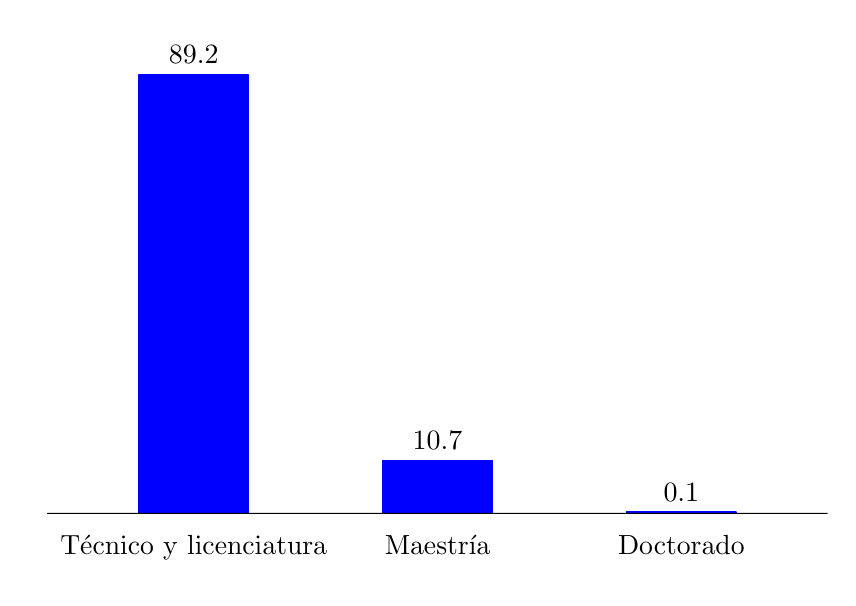
\begin{tikzpicture}[x=1pt,y=1pt]  % Created by tikzDevice version 0.7.0 on 2015-08-28 14:02:54
% !TEX encoding = UTF-8 Unicode
\definecolor[named]{fillColor}{rgb}{1.00,1.00,1.00}
\path[use as bounding box,fill=fillColor,fill opacity=0.00] (0,0) rectangle (289.08,198.74);
\begin{scope}
\path[clip] (  0.00,  0.00) rectangle (289.08,198.74);
\definecolor[named]{drawColor}{rgb}{1.00,1.00,1.00}

\path[draw=drawColor,line width= 0.6pt,line join=round,line cap=round] (  0.00,  0.00) rectangle (289.08,198.74);
\end{scope}
\begin{scope}
\path[clip] (  0.00,  0.00) rectangle (289.08,198.74);

\path[] (  7.11, 23.47) rectangle (289.08,181.67);

\path[] ( 59.98, 23.47) --
	( 59.98,181.67);

\path[] (148.10, 23.47) --
	(148.10,181.67);

\path[] (236.21, 23.47) --
	(236.21,181.67);
\definecolor[named]{drawColor}{rgb}{0.00,0.00,1.00}
\definecolor[named]{fillColor}{rgb}{0.00,0.00,1.00}

\path[draw=drawColor,line width= 0.6pt,line join=round,fill=fillColor] ( 40.16, 23.47) rectangle ( 79.81,181.67);

\path[draw=drawColor,line width= 0.6pt,line join=round,fill=fillColor] (128.27, 23.47) rectangle (167.92, 42.36);

\path[draw=drawColor,line width= 0.6pt,line join=round,fill=fillColor] (216.39, 23.47) rectangle (256.04, 23.73);
\definecolor[named]{drawColor}{rgb}{0.00,0.00,0.00}
\definecolor[named]{fillColor}{rgb}{0.00,0.00,0.00}

\path[draw=drawColor,line width= 0.1pt,line join=round,fill=fillColor] (  7.11, 23.47) -- (289.08, 23.47);

\node[text=drawColor,anchor=base,inner sep=0pt, outer sep=0pt, scale=  1.01] at ( 59.98,185.63) {89.2};

\node[text=drawColor,anchor=base,inner sep=0pt, outer sep=0pt, scale=  1.01] at (148.10, 46.32) {10.7};

\node[text=drawColor,anchor=base,inner sep=0pt, outer sep=0pt, scale=  1.01] at (236.21, 27.68) {0.1};
\end{scope}
\begin{scope}
\path[clip] (  0.00,  0.00) rectangle (289.08,198.74);

\path[] (  7.11, 23.47) --
	(  7.11,181.67);
\end{scope}
\begin{scope}
\path[clip] (  0.00,  0.00) rectangle (289.08,198.74);

\path[] (  7.11, 23.47) --
	(289.08, 23.47);
\end{scope}
\begin{scope}
\path[clip] (  0.00,  0.00) rectangle (289.08,198.74);

\path[] ( 59.98, 19.20) --
	( 59.98, 23.47);

\path[] (148.10, 19.20) --
	(148.10, 23.47);

\path[] (236.21, 19.20) --
	(236.21, 23.47);
\end{scope}
\begin{scope}
\path[clip] (  0.00,  0.00) rectangle (289.08,198.74);
\definecolor[named]{drawColor}{rgb}{0.00,0.00,0.00}

\node[text=drawColor,anchor=base,inner sep=0pt, outer sep=0pt, scale=  1.00] at ( 59.98,  8.54) {T\'ecnico y licenciatura};

\node[text=drawColor,anchor=base,inner sep=0pt, outer sep=0pt, scale=  1.00] at (148.10,  8.54) {Maestr\'ia};

\node[text=drawColor,anchor=base,inner sep=0pt, outer sep=0pt, scale=  1.00] at (236.21,  8.54) {Doctorado};
\end{scope}
  \end{tikzpicture}}{Instituto Nacional de Estadística}


\cajita{Evolución del gasto en educación, por entidad}{Del gasto público total asignado en el 2013, el Ministerio de Educación recibió un 78\%. En el 2012 había recibido el 77\%.\\
	
	La segunda y tercer mayor asignación fue para dos entidades descentralizadas, la Universidad de San Carlos de Guatemala (que  tuvo un crecimiento presupuestario del 4\% respecto al 2012)\textollamada[*]{Los cálculos están realizados en quetzales corrientes de cada año.}, y el Instituto Técnico de Capacitación y Productividad.}{Gasto público en educación, por entidad}{República de Guatemala, 2012 y 2013, en millones de quetzales de cada año}{
	\ra{1.2}$\ $\\
	\begin{tabular}{p{6cm}rr}\hline
		\rowcolor{color2!15!white} &&\\[-4mm]
		{\Bold    Entidad          }&       \textbf{2012}   &   \textbf{2013}    \\
		\rowcolor{white} &&\\[-4mm]
		
	\textbf{	Total }&\textbf{	12,133} &\textbf{	12,896} \\
	Ministerio de Educación	& 9,342 &	10,003 \\
		Universidad de San Carlos&	1,568 &	1,627 \\
		Instituto Técnico de Capacitación y Productividad&	230 &	256 \\
		Obligaciones del Estado a cargo del Tesoro&	279 &	189 \\
		Comité Nacional de Alfabetización&	129 &	188 \\
		Ministerio de la Defensa Nacional&	159 &	182 \\
		Ministerio de Salud Pública y Asistencia Social&	178 &	154 \\
		Ministerio de Gobernación&	60& 	129 \\
		Escuela Nacional Central de Agricultura&	33& 	46 \\
		Resto de entidades&	155&	122\\
		
		\hline
		\rowcolor{white} &&\\[-5.5mm]

		&&\\[-0.09cm]
	\end{tabular}}{Instituto Nacional de Estadística}


\cajita{Gasto por entidad}{Del total de gasto público en educación asignado a entidades centralizadas (83.3\% del total de gasto público), el 93\% se destina al Ministerio de Educación.
	
	 Del mismo El 22.4\% del gasto público en educación es asignado a las La distribución porcentual del gasto público en educación }{Distribución del gasto público en educación por entidad}{República de Guatemala, 2013, en porcentaje}{\ \\[0mm]\begin{tikzpicture}[x=1pt,y=1pt]  % Created by tikzDevice version 0.7.0 on 2015-09-01 14:31:10
% !TEX encoding = UTF-8 Unicode
\definecolor[named]{fillColor}{rgb}{1.00,1.00,1.00}
\path[use as bounding box,fill=fillColor,fill opacity=0.00] (0,0) rectangle (289.08,198.74);
\begin{scope}
\path[clip] (  0.00,  0.00) rectangle (289.08,198.74);
\definecolor[named]{drawColor}{rgb}{1.00,1.00,1.00}

\path[draw=drawColor,line width= 0.6pt,line join=round,line cap=round] (  0.00,  0.00) rectangle (289.08,198.74);
\end{scope}
\begin{scope}
\path[clip] (  0.00,  0.00) rectangle (289.08,198.74);

\path[] ( -2.73, 17.78) rectangle (280.54,191.48);

\path[] (  0.00, 54.05) --
	(280.54, 54.05);

\path[] (  0.00,110.80) --
	(280.54,110.80);

\path[] (  0.00,167.55) --
	(280.54,167.55);

\path[] (  0.00, 25.67) --
	(280.54, 25.67);

\path[] (  0.00, 82.42) --
	(280.54, 82.42);

\path[] (  0.00,139.17) --
	(280.54,139.17);

\path[] ( 37.73, 17.78) --
	( 37.73,191.48);

\path[] (105.18, 17.78) --
	(105.18,191.48);

\path[] (172.63, 17.78) --
	(172.63,191.48);

\path[] (240.08, 17.78) --
	(240.08,191.48);
\definecolor[named]{drawColor}{rgb}{0.00,0.00,1.00}

\path[draw=drawColor,line width= 1.7pt,line join=round] ( 37.73,182.20) --
	(105.18,180.01) --
	(172.63,183.59) --
	(240.08,178.90);
\definecolor[named]{drawColor}{rgb}{0.00,0.00,0.00}

\node[text=drawColor,anchor=base,inner sep=0pt, outer sep=0pt, scale=  1.01] at ( 37.73,186.15) {3.8};

\node[text=drawColor,anchor=base,inner sep=0pt, outer sep=0pt, scale=  1.01] at (105.18,168.14) {3.7};

\node[text=drawColor,anchor=base,inner sep=0pt, outer sep=0pt, scale=  1.01] at (172.63,187.54) {3.8};

\node[text=drawColor,anchor=base,inner sep=0pt, outer sep=0pt, scale=  1.01] at (240.08,167.03) {3.7};
\definecolor[named]{fillColor}{rgb}{0.00,0.00,0.00}

\path[draw=drawColor,line width= 0.1pt,line join=round,fill=fillColor] (  0.00, 25.67) -- (280.54, 25.67);
\end{scope}
\begin{scope}
\path[clip] (  0.00,  0.00) rectangle (289.08,198.74);

\path[] (  0.00, 17.78) --
	(280.54, 17.78);
\end{scope}
\begin{scope}
\path[clip] (  0.00,  0.00) rectangle (289.08,198.74);

\path[] ( 37.73, 13.51) --
	( 37.73, 17.78);

\path[] (105.18, 13.51) --
	(105.18, 17.78);

\path[] (172.63, 13.51) --
	(172.63, 17.78);

\path[] (240.08, 13.51) --
	(240.08, 17.78);
\end{scope}
\begin{scope}
\path[clip] (  0.00,  0.00) rectangle (289.08,198.74);
\definecolor[named]{drawColor}{rgb}{0.00,0.00,0.00}

\node[text=drawColor,anchor=base,inner sep=0pt, outer sep=0pt, scale=  1.00] at ( 37.73,  2.85) {2010};

\node[text=drawColor,anchor=base,inner sep=0pt, outer sep=0pt, scale=  1.00] at (105.18,  2.85) {2011};

\node[text=drawColor,anchor=base,inner sep=0pt, outer sep=0pt, scale=  1.00] at (172.63,  2.85) {2012};

\node[text=drawColor,anchor=base,inner sep=0pt, outer sep=0pt, scale=  1.00] at (240.08,  2.85) {2013};
\end{scope}
  \end{tikzpicture}}{Instituto Nacional de Estadística}


\cajita{Crecimiento del gasto en educación por entidad}{De las entidades con mayor erogación de gasto público, tuvieron  mayor crecimiento de gasto, respecto al 2012, el Ministerio de Gobernación con el 115.7\%, seguido del Comité Nacional de Alfabetización 45.7\%. 
	
\textollamada[*]{La tasa de crecimiento se calculó utilizando quetzales corrientes de 2012 y 2013.}	Las entidades con mayor decrecimiento fueron las obligaciones del Estado a cargo del Tesoro 32.2\% y el Ministerio de Salud Pública y Asistencia Social 13.1\%.}{Tasa de crecimiento anual del gasto público en educación, por entidades con mayor erogación}{República de Guatemala, 2013, en porcentaje}{\ \\[0mm]\begin{tikzpicture}[x=1pt,y=1pt]  % Created by tikzDevice version 0.7.0 on 2015-08-28 16:54:23
% !TEX encoding = UTF-8 Unicode
\definecolor[named]{fillColor}{rgb}{1.00,1.00,1.00}
\path[use as bounding box,fill=fillColor,fill opacity=0.00] (0,0) rectangle (289.08,198.74);
\begin{scope}
\path[clip] (  0.00,  0.00) rectangle (289.08,198.74);
\definecolor[named]{drawColor}{rgb}{1.00,1.00,1.00}

\path[draw=drawColor,line width= 0.6pt,line join=round,line cap=round] (  0.00,  0.00) rectangle (289.08,198.74);
\end{scope}
\begin{scope}
\path[clip] (  0.00,  0.00) rectangle (289.08,198.74);

\path[] (  7.11, 32.50) rectangle (289.08,174.70);

\path[] ( 34.40, 32.50) --
	( 34.40,174.70);

\path[] ( 79.88, 32.50) --
	( 79.88,174.70);

\path[] (125.36, 32.50) --
	(125.36,174.70);

\path[] (170.84, 32.50) --
	(170.84,174.70);

\path[] (216.31, 32.50) --
	(216.31,174.70);

\path[] (261.79, 32.50) --
	(261.79,174.70);
\definecolor[named]{drawColor}{rgb}{0.00,0.00,1.00}
\definecolor[named]{fillColor}{rgb}{0.00,0.00,1.00}

\path[draw=drawColor,line width= 0.6pt,line join=round,fill=fillColor] ( 16.66, 32.50) rectangle ( 31.67, 36.87);
\definecolor[named]{drawColor}{rgb}{0.62,0.73,1.00}
\definecolor[named]{fillColor}{rgb}{0.62,0.73,1.00}

\path[draw=drawColor,line width= 0.6pt,line join=round,fill=fillColor] ( 37.13, 32.50) rectangle ( 52.14, 33.81);
\definecolor[named]{drawColor}{rgb}{0.00,0.00,1.00}
\definecolor[named]{fillColor}{rgb}{0.00,0.00,1.00}

\path[draw=drawColor,line width= 0.6pt,line join=round,fill=fillColor] ( 62.14, 32.50) rectangle ( 77.15, 54.13);
\definecolor[named]{drawColor}{rgb}{0.62,0.73,1.00}
\definecolor[named]{fillColor}{rgb}{0.62,0.73,1.00}

\path[draw=drawColor,line width= 0.6pt,line join=round,fill=fillColor] ( 82.61, 32.50) rectangle ( 97.62, 63.30);
\definecolor[named]{drawColor}{rgb}{0.00,0.00,1.00}
\definecolor[named]{fillColor}{rgb}{0.00,0.00,1.00}

\path[draw=drawColor,line width= 0.6pt,line join=round,fill=fillColor] (107.62, 32.50) rectangle (122.63, 54.34);
\definecolor[named]{drawColor}{rgb}{0.62,0.73,1.00}
\definecolor[named]{fillColor}{rgb}{0.62,0.73,1.00}

\path[draw=drawColor,line width= 0.6pt,line join=round,fill=fillColor] (128.09, 32.50) rectangle (143.09, 48.01);
\definecolor[named]{drawColor}{rgb}{0.00,0.00,1.00}
\definecolor[named]{fillColor}{rgb}{0.00,0.00,1.00}

\path[draw=drawColor,line width= 0.6pt,line join=round,fill=fillColor] (153.10, 32.50) rectangle (168.11, 35.34);
\definecolor[named]{drawColor}{rgb}{0.62,0.73,1.00}
\definecolor[named]{fillColor}{rgb}{0.62,0.73,1.00}

\path[draw=drawColor,line width= 0.6pt,line join=round,fill=fillColor] (173.56, 32.50) rectangle (188.57, 32.50);
\definecolor[named]{drawColor}{rgb}{0.00,0.00,1.00}
\definecolor[named]{fillColor}{rgb}{0.00,0.00,1.00}

\path[draw=drawColor,line width= 0.6pt,line join=round,fill=fillColor] (198.58, 32.50) rectangle (213.59,138.44);
\definecolor[named]{drawColor}{rgb}{0.62,0.73,1.00}
\definecolor[named]{fillColor}{rgb}{0.62,0.73,1.00}

\path[draw=drawColor,line width= 0.6pt,line join=round,fill=fillColor] (219.04, 32.50) rectangle (234.05,174.70);
\definecolor[named]{drawColor}{rgb}{0.00,0.00,1.00}
\definecolor[named]{fillColor}{rgb}{0.00,0.00,1.00}

\path[draw=drawColor,line width= 0.6pt,line join=round,fill=fillColor] (244.06, 32.50) rectangle (259.06, 94.32);
\definecolor[named]{drawColor}{rgb}{0.62,0.73,1.00}
\definecolor[named]{fillColor}{rgb}{0.62,0.73,1.00}

\path[draw=drawColor,line width= 0.6pt,line join=round,fill=fillColor] (264.52, 32.50) rectangle (279.53, 61.12);
\definecolor[named]{drawColor}{rgb}{0.00,0.00,0.00}
\definecolor[named]{fillColor}{rgb}{0.00,0.00,0.00}

\path[draw=drawColor,line width= 0.6pt,line join=round,fill=fillColor] (  7.11, 32.50) -- (289.08, 32.50);

\node[text=drawColor,anchor=base,inner sep=0pt, outer sep=0pt, scale=  0.82] at ( 24.17, 40.09) {2.0};

\node[text=drawColor,anchor=base,inner sep=0pt, outer sep=0pt, scale=  0.82] at ( 44.63, 37.03) {0.6};

\node[text=drawColor,anchor=base,inner sep=0pt, outer sep=0pt, scale=  0.82] at ( 69.65, 57.35) {9.9};

\node[text=drawColor,anchor=base,inner sep=0pt, outer sep=0pt, scale=  0.82] at ( 90.11, 66.52) {14.1};

\node[text=drawColor,anchor=base,inner sep=0pt, outer sep=0pt, scale=  0.82] at (115.12, 57.57) {10.0};

\node[text=drawColor,anchor=base,inner sep=0pt, outer sep=0pt, scale=  0.82] at (135.59, 51.23) {7.1};

\node[text=drawColor,anchor=base,inner sep=0pt, outer sep=0pt, scale=  0.82] at (160.60, 38.56) {1.3};

\node[text=drawColor,anchor=base,inner sep=0pt, outer sep=0pt, scale=  0.82] at (181.07, 35.72) {0.0};

\node[text=drawColor,anchor=base,inner sep=0pt, outer sep=0pt, scale=  0.82] at (206.08,141.67) {48.5};

\node[text=drawColor,anchor=base,inner sep=0pt, outer sep=0pt, scale=  0.82] at (226.55,177.93) {65.1};

\node[text=drawColor,anchor=base,inner sep=0pt, outer sep=0pt, scale=  0.82] at (251.56, 97.54) {28.3};

\node[text=drawColor,anchor=base,inner sep=0pt, outer sep=0pt, scale=  0.82] at (272.03, 64.34) {13.1};
\end{scope}
\begin{scope}
\path[clip] (  0.00,  0.00) rectangle (289.08,198.74);

\path[] (  7.11, 32.50) --
	(  7.11,174.70);
\end{scope}
\begin{scope}
\path[clip] (  0.00,  0.00) rectangle (289.08,198.74);

\path[] (  7.11, 32.50) --
	(289.08, 32.50);
\end{scope}
\begin{scope}
\path[clip] (  0.00,  0.00) rectangle (289.08,198.74);

\path[] ( 34.40, 28.23) --
	( 34.40, 32.50);

\path[] ( 79.88, 28.23) --
	( 79.88, 32.50);

\path[] (125.36, 28.23) --
	(125.36, 32.50);

\path[] (170.84, 28.23) --
	(170.84, 32.50);

\path[] (216.31, 28.23) --
	(216.31, 32.50);

\path[] (261.79, 28.23) --
	(261.79, 32.50);
\end{scope}
\begin{scope}
\path[clip] (  0.00,  0.00) rectangle (289.08,198.74);
\definecolor[named]{drawColor}{rgb}{0.00,0.00,0.00}

\node[text=drawColor,anchor=base,inner sep=0pt, outer sep=0pt, scale=  1.00] at ( 34.40, 17.57) {Ciencias};

\node[text=drawColor,anchor=base,inner sep=0pt, outer sep=0pt, scale=  1.00] at ( 34.40,  5.69) { naturales};

\node[text=drawColor,anchor=base,inner sep=0pt, outer sep=0pt, scale=  1.00] at ( 79.88, 17.57) {Ingenier\'ias};

\node[text=drawColor,anchor=base,inner sep=0pt, outer sep=0pt, scale=  1.00] at ( 79.88,  5.69) { y tecnolog\'ia};

\node[text=drawColor,anchor=base,inner sep=0pt, outer sep=0pt, scale=  1.00] at (125.36, 17.57) {Ciencias};

\node[text=drawColor,anchor=base,inner sep=0pt, outer sep=0pt, scale=  1.00] at (125.36,  5.69) { m\'edicas};

\node[text=drawColor,anchor=base,inner sep=0pt, outer sep=0pt, scale=  1.00] at (170.84, 17.57) {Ciencias};

\node[text=drawColor,anchor=base,inner sep=0pt, outer sep=0pt, scale=  1.00] at (170.84,  5.69) { agr\'icolas};

\node[text=drawColor,anchor=base,inner sep=0pt, outer sep=0pt, scale=  1.00] at (216.31, 17.57) {Ciencias};

\node[text=drawColor,anchor=base,inner sep=0pt, outer sep=0pt, scale=  1.00] at (216.31,  5.69) { sociales};

\node[text=drawColor,anchor=base,inner sep=0pt, outer sep=0pt, scale=  1.00] at (261.79, 11.63) {Humanidades};
\end{scope}
\coordinate (apoyo) at (57.37,191.07);
\coordinate (longitudFicticia) at (7.11,7.67);
\coordinate (longitud) at (7.11,7.11);
\coordinate (desX) at (138.52,0);
\coordinate (desY) at (0,0.28);
\definecolor[named]{ct1}{HTML}{
0000FF
}
\definecolor[named]{ct2}{HTML}{
9DBBFF
}
\definecolor[named]{ctb1}{HTML}{
0000FF
}
\definecolor[named]{ctb2}{HTML}{
9DBBFF
}
\path [fill=none] (apoyo) rectangle ($(apoyo)+(longitudFicticia)$)
node [xshift=0.3cm,inner sep=0pt, outer sep=0pt,midway,right,scale = 0.9]{P\'ublico};
\draw [color = ctb1,fill=ct1] ( $(apoyo)  + (desY) $) rectangle ($(apoyo)+ (desY) +(longitud)$);
\path [fill=none] ($(apoyo)+(desX)$) rectangle ($(apoyo)+(desX)+(longitudFicticia)$)
node [xshift=0.3cm,inner sep=0pt, outer sep=0pt,midway,right,scale = 0.9]{Privado};
\draw [color = ctb2 ,fill=ct2] ( $(apoyo)  + (desY) + (desX) $) rectangle ($(apoyo)+ (desY)+ (desX) +(longitud)$);
  \end{tikzpicture}}{Instituto Nacional de Estadística}


\cajita{Evolución del gasto en educación, por grupo}{Según el grupo de gasto, el pago en servicios personales y no personales abarcó en el 2013 el 84\% del gasto público en educación. \\
	
	El grupo de gasto de materiales y suministro tuvo una disminución del 31\% respecto a la asignación del 2012.}{Gasto público en educación, por grupo de gasto}{República de Guatemala, 2012 y 2013, en millones de quetzales de cada año}{
	\ra{1.2}$\ $\\
	\begin{tabular}{p{6cm}rr}\hline
		\rowcolor{color2!15!white} &&\\[-4mm]
		{\Bold    Grupo de gasto         }&      \textbf{2012}   &  \textbf{2013}    \\
\hline
		\rowcolor{white} &&\\[-4mm]
		
\textbf{	Total}&	\textbf{12,133}& 	\textbf{12,896 }\\
	Servicios Personales&	9,344 &	10,272 \\
	Servicios No Personales&	653 &	597 \\
	Materiales y Suministros&	859 &	590 \\
	Propiedad, Planta, Equipo e Intangibles&	207& 	204 \\
	Transferencias Corrientes&	777 &	1,027 \\
	Transferencias de Capital&	276 &	189 \\
	Asignaciones Globales&	16 &	17 \\
			\hline
		\rowcolor{white} &&\\[-5.5mm]
	
		&&\\[-0.09cm]
	\end{tabular}}{Instituto Nacional de Estadística}


\cajita{Gasto en educación por grupo}{El rubro más importante, en relación a la cantidad en la asignación de gasto, ha sido el pago de servicios personales, que representa el 79.7\% del total del gasto público en educación. Los materiales y suministros representaron el 4.6\% del gasto total.}{Distribución del gasto público en educación por grupo de gasto}{República de Guatemala, 2013, en porcentaje}{\ \\[0mm]\begin{tikzpicture}[x=1pt,y=1pt]  % Created by tikzDevice version 0.7.0 on 2015-08-28 14:35:24
% !TEX encoding = UTF-8 Unicode
\definecolor[named]{fillColor}{rgb}{1.00,1.00,1.00}
\path[use as bounding box,fill=fillColor,fill opacity=0.00] (0,0) rectangle (289.08,198.74);
\begin{scope}
\path[clip] (  0.00,  0.00) rectangle (289.08,198.74);
\definecolor[named]{drawColor}{rgb}{1.00,1.00,1.00}

\path[draw=drawColor,line width= 0.6pt,line join=round,line cap=round] (  0.00,  0.00) rectangle (289.08,198.74);
\end{scope}
\begin{scope}
\path[clip] (  0.00,  0.00) rectangle (289.08,198.74);

\path[] (  1.64, 17.78) rectangle (280.54,191.48);

\path[] (  1.64, 44.19) --
	(280.54, 44.19);

\path[] (  1.64, 81.22) --
	(280.54, 81.22);

\path[] (  1.64,118.25) --
	(280.54,118.25);

\path[] (  1.64,155.28) --
	(280.54,155.28);

\path[] (  1.64, 25.67) --
	(280.54, 25.67);

\path[] (  1.64, 62.70) --
	(280.54, 62.70);

\path[] (  1.64, 99.73) --
	(280.54, 99.73);

\path[] (  1.64,136.76) --
	(280.54,136.76);

\path[] (  1.64,173.79) --
	(280.54,173.79);

\path[] ( 41.49, 17.78) --
	( 41.49,191.48);

\path[] (107.89, 17.78) --
	(107.89,191.48);

\path[] (174.30, 17.78) --
	(174.30,191.48);

\path[] (240.70, 17.78) --
	(240.70,191.48);
\definecolor[named]{drawColor}{rgb}{0.00,0.00,1.00}

\path[draw=drawColor,line width= 1.7pt,line join=round] ( 41.49,151.95) --
	(107.89,166.39) --
	(174.30,168.98) --
	(240.70,183.59);
\definecolor[named]{drawColor}{rgb}{0.00,0.00,0.00}

\node[text=drawColor,anchor=base,inner sep=0pt, outer sep=0pt, scale=  1.01] at ( 41.49,140.08) {34.1};

\node[text=drawColor,anchor=base east,inner sep=0pt, outer sep=0pt, scale=  1.01] at (104.78,166.39) {38.0};

\node[text=drawColor,anchor=base east,inner sep=0pt, outer sep=0pt, scale=  1.01] at (171.18,168.98) {38.7};

\node[text=drawColor,anchor=base,inner sep=0pt, outer sep=0pt, scale=  1.01] at (240.70,187.54) {42.6};
\definecolor[named]{fillColor}{rgb}{0.00,0.00,0.00}

\path[draw=drawColor,line width= 0.1pt,line join=round,fill=fillColor] (  1.64, 25.67) -- (280.54, 25.67);
\end{scope}
\begin{scope}
\path[clip] (  0.00,  0.00) rectangle (289.08,198.74);

\path[] (  1.64, 17.78) --
	(  1.64,191.48);
\end{scope}
\begin{scope}
\path[clip] (  0.00,  0.00) rectangle (289.08,198.74);

\path[] (  0.00, 25.67) --
	(  1.64, 25.67);

\path[] (  0.00, 62.70) --
	(  1.64, 62.70);

\path[] (  0.00, 99.73) --
	(  1.64, 99.73);

\path[] (  0.00,136.76) --
	(  1.64,136.76);

\path[] (  0.00,173.79) --
	(  1.64,173.79);
\end{scope}
\begin{scope}
\path[clip] (  0.00,  0.00) rectangle (289.08,198.74);

\path[] (  1.64, 17.78) --
	(280.54, 17.78);
\end{scope}
\begin{scope}
\path[clip] (  0.00,  0.00) rectangle (289.08,198.74);

\path[] ( 41.49, 13.51) --
	( 41.49, 17.78);

\path[] (107.89, 13.51) --
	(107.89, 17.78);

\path[] (174.30, 13.51) --
	(174.30, 17.78);

\path[] (240.70, 13.51) --
	(240.70, 17.78);
\end{scope}
\begin{scope}
\path[clip] (  0.00,  0.00) rectangle (289.08,198.74);
\definecolor[named]{drawColor}{rgb}{0.00,0.00,0.00}

\node[text=drawColor,anchor=base,inner sep=0pt, outer sep=0pt, scale=  1.00] at ( 41.49,  2.85) {2010};

\node[text=drawColor,anchor=base,inner sep=0pt, outer sep=0pt, scale=  1.00] at (107.89,  2.85) {2011};

\node[text=drawColor,anchor=base,inner sep=0pt, outer sep=0pt, scale=  1.00] at (174.30,  2.85) {2012};

\node[text=drawColor,anchor=base,inner sep=0pt, outer sep=0pt, scale=  1.00] at (240.70,  2.85) {2013};
\end{scope}
  \end{tikzpicture}}{Instituto Nacional de Estadística}


\cajita{Crecimiento del gasto en educación por grupo}{\textollamada[*]{Los cálculos están realizados en quetzales corrientes de cada año.}El rubro que tuvo un mayor crecimiento de gasto, respecto al 2012, fueron las transferencias corrientes, con el 32.2\%, seguido de los servicios personales con el 9.9\%. El rubro con el mayor decrecimiento fueron las transferencias de capital, con el 31.5\% y el rubro de materiales y suministros con el 31.4\%.}{Tasa de crecimiento anual del gasto público en educación por grupo de gasto}{República de Guatemala, 2013, en porcentaje}{\ \\[0mm]\begin{tikzpicture}[x=1pt,y=1pt]  % Created by tikzDevice version 0.7.0 on 2015-08-28 14:52:30
% !TEX encoding = UTF-8 Unicode
\definecolor[named]{fillColor}{rgb}{1.00,1.00,1.00}
\path[use as bounding box,fill=fillColor,fill opacity=0.00] (0,0) rectangle (289.08,198.74);
\begin{scope}
\path[clip] (  0.00,  0.00) rectangle (289.08,198.74);
\definecolor[named]{drawColor}{rgb}{1.00,1.00,1.00}

\path[draw=drawColor,line width= 0.6pt,line join=round,line cap=round] (  0.00,  0.00) rectangle (289.08,198.74);
\end{scope}
\begin{scope}
\path[clip] (  0.00,  0.00) rectangle (289.08,198.74);

\path[] (  7.11, 20.62) rectangle (289.08,174.77);

\path[] ( 39.65, 20.62) --
	( 39.65,174.77);

\path[] ( 93.87, 20.62) --
	( 93.87,174.77);

\path[] (148.10, 20.62) --
	(148.10,174.77);

\path[] (202.32, 20.62) --
	(202.32,174.77);

\path[] (256.55, 20.62) --
	(256.55,174.77);
\definecolor[named]{drawColor}{rgb}{0.00,0.00,1.00}
\definecolor[named]{fillColor}{rgb}{0.00,0.00,1.00}

\path[draw=drawColor,line width= 0.6pt,line join=round,fill=fillColor] ( 18.64, 20.62) rectangle ( 36.26,172.59);
\definecolor[named]{drawColor}{rgb}{0.62,0.73,1.00}
\definecolor[named]{fillColor}{rgb}{0.62,0.73,1.00}

\path[draw=drawColor,line width= 0.6pt,line join=round,fill=fillColor] ( 43.04, 20.62) rectangle ( 60.66,155.23);
\definecolor[named]{drawColor}{rgb}{0.00,0.00,1.00}
\definecolor[named]{fillColor}{rgb}{0.00,0.00,1.00}

\path[draw=drawColor,line width= 0.6pt,line join=round,fill=fillColor] ( 72.86, 20.62) rectangle ( 90.48,174.77);
\definecolor[named]{drawColor}{rgb}{0.62,0.73,1.00}
\definecolor[named]{fillColor}{rgb}{0.62,0.73,1.00}

\path[draw=drawColor,line width= 0.6pt,line join=round,fill=fillColor] ( 97.26, 20.62) rectangle (114.88,142.20);
\definecolor[named]{drawColor}{rgb}{0.00,0.00,1.00}
\definecolor[named]{fillColor}{rgb}{0.00,0.00,1.00}

\path[draw=drawColor,line width= 0.6pt,line join=round,fill=fillColor] (127.08, 20.62) rectangle (144.71,168.25);
\definecolor[named]{drawColor}{rgb}{0.62,0.73,1.00}
\definecolor[named]{fillColor}{rgb}{0.62,0.73,1.00}

\path[draw=drawColor,line width= 0.6pt,line join=round,fill=fillColor] (151.49, 20.62) rectangle (169.11,144.37);
\definecolor[named]{drawColor}{rgb}{0.00,0.00,1.00}
\definecolor[named]{fillColor}{rgb}{0.00,0.00,1.00}

\path[draw=drawColor,line width= 0.6pt,line join=round,fill=fillColor] (181.31, 20.62) rectangle (198.93,159.57);
\definecolor[named]{drawColor}{rgb}{0.62,0.73,1.00}
\definecolor[named]{fillColor}{rgb}{0.62,0.73,1.00}

\path[draw=drawColor,line width= 0.6pt,line join=round,fill=fillColor] (205.71, 20.62) rectangle (223.33,135.69);
\definecolor[named]{drawColor}{rgb}{0.00,0.00,1.00}
\definecolor[named]{fillColor}{rgb}{0.00,0.00,1.00}

\path[draw=drawColor,line width= 0.6pt,line join=round,fill=fillColor] (235.53, 20.62) rectangle (253.16,133.52);
\definecolor[named]{drawColor}{rgb}{0.62,0.73,1.00}
\definecolor[named]{fillColor}{rgb}{0.62,0.73,1.00}

\path[draw=drawColor,line width= 0.6pt,line join=round,fill=fillColor] (259.93, 20.62) rectangle (277.56,111.81);
\definecolor[named]{drawColor}{rgb}{0.00,0.00,0.00}
\definecolor[named]{fillColor}{rgb}{0.00,0.00,0.00}

\path[draw=drawColor,line width= 0.6pt,line join=round,fill=fillColor] (  7.11, 20.62) -- (289.08, 20.62);

\node[text=drawColor,anchor=base,inner sep=0pt, outer sep=0pt, scale=  0.82] at ( 27.45,175.82) {7.0};

\node[text=drawColor,anchor=base,inner sep=0pt, outer sep=0pt, scale=  0.82] at ( 51.85,158.45) {6.2};

\node[text=drawColor,anchor=base,inner sep=0pt, outer sep=0pt, scale=  0.82] at ( 81.67,177.99) {7.1};

\node[text=drawColor,anchor=base,inner sep=0pt, outer sep=0pt, scale=  0.82] at (106.07,145.42) {5.6};

\node[text=drawColor,anchor=base,inner sep=0pt, outer sep=0pt, scale=  0.82] at (135.90,171.48) {6.8};

\node[text=drawColor,anchor=base,inner sep=0pt, outer sep=0pt, scale=  0.82] at (160.30,147.59) {5.7};

\node[text=drawColor,anchor=base,inner sep=0pt, outer sep=0pt, scale=  0.82] at (190.12,162.79) {6.4};

\node[text=drawColor,anchor=base,inner sep=0pt, outer sep=0pt, scale=  0.82] at (214.52,138.91) {5.3};

\node[text=drawColor,anchor=base,inner sep=0pt, outer sep=0pt, scale=  0.82] at (244.34,136.74) {5.2};

\node[text=drawColor,anchor=base,inner sep=0pt, outer sep=0pt, scale=  0.82] at (268.75,115.03) {4.2};
\end{scope}
\begin{scope}
\path[clip] (  0.00,  0.00) rectangle (289.08,198.74);

\path[] (  7.11, 20.62) --
	(  7.11,174.77);
\end{scope}
\begin{scope}
\path[clip] (  0.00,  0.00) rectangle (289.08,198.74);

\path[] (  7.11, 20.62) --
	(289.08, 20.62);
\end{scope}
\begin{scope}
\path[clip] (  0.00,  0.00) rectangle (289.08,198.74);

\path[] ( 39.65, 16.35) --
	( 39.65, 20.62);

\path[] ( 93.87, 16.35) --
	( 93.87, 20.62);

\path[] (148.10, 16.35) --
	(148.10, 20.62);

\path[] (202.32, 16.35) --
	(202.32, 20.62);

\path[] (256.55, 16.35) --
	(256.55, 20.62);
\end{scope}
\begin{scope}
\path[clip] (  0.00,  0.00) rectangle (289.08,198.74);
\definecolor[named]{drawColor}{rgb}{0.00,0.00,0.00}

\node[text=drawColor,anchor=base,inner sep=0pt, outer sep=0pt, scale=  1.00] at ( 39.65,  5.69) {1987};

\node[text=drawColor,anchor=base,inner sep=0pt, outer sep=0pt, scale=  1.00] at ( 93.87,  5.69) {1995};

\node[text=drawColor,anchor=base,inner sep=0pt, outer sep=0pt, scale=  1.00] at (148.10,  5.69) {1998/99};

\node[text=drawColor,anchor=base,inner sep=0pt, outer sep=0pt, scale=  1.00] at (202.32,  5.69) {2002};

\node[text=drawColor,anchor=base,inner sep=0pt, outer sep=0pt, scale=  1.00] at (256.55,  5.69) {2008/09};
\end{scope}
\coordinate (apoyo) at (50.29,191.13);
\coordinate (longitudFicticia) at (7.11,7.61);
\coordinate (longitud) at (7.11,7.11);
\coordinate (desX) at (142.09,0);
\coordinate (desY) at (0,0.25);
\definecolor[named]{ct1}{HTML}{
0000FF
}
\definecolor[named]{ct2}{HTML}{
9DBBFF
}
\definecolor[named]{ctb1}{HTML}{
0000FF
}
\definecolor[named]{ctb2}{HTML}{
9DBBFF
}
\path [fill=none] (apoyo) rectangle ($(apoyo)+(longitudFicticia)$)
node [xshift=0.3cm,inner sep=0pt, outer sep=0pt,midway,right,scale = 0.9]{Observados};
\draw [color = ctb1,fill=ct1] ( $(apoyo)  + (desY) $) rectangle ($(apoyo)+ (desY) +(longitud)$);
\path [fill=none] ($(apoyo)+(desX)$) rectangle ($(apoyo)+(desX)+(longitudFicticia)$)
node [xshift=0.3cm,inner sep=0pt, outer sep=0pt,midway,right,scale = 0.9]{Deseados};
\draw [color = ctb2 ,fill=ct2] ( $(apoyo)  + (desY) + (desX) $) rectangle ($(apoyo)+ (desY)+ (desX) +(longitud)$);
  \end{tikzpicture}}{Instituto Nacional de Estadística}


\cajita{Evolución del gasto en educación, por tipo}{El gasto público en educación se puede dividir en gastos corrientes y gastos de capital. En el corriente se incluyen el pago de salarios a funcionarios, compras de bienes y servicios, el cual representó 97\% de la asignación en gasto en educación.}{Gasto público en educación por tipo de gasto}{República de Guatemala, 2012 y 2013, en millones de quetzales de cada año}{
	\ra{1.2}$\ $\\
	\begin{tabular}{p{6cm}rr}\hline
		\rowcolor{color2!15!white} &&\\[-4mm]
		{\Bold    Tipo de gasto         }&     \textbf{  2012 }  &  \textbf{ 2013 }   \\
		\hline
		\rowcolor{white} &&\\[-4mm]
		
	\textbf{Total}&	\textbf{12,133}&	\textbf{12,896}\\
	Gastos Corrientes&	11,649	& 12,499\\
	Gastos de Capital&	484	& 398\\	
		\hline
		\rowcolor{white} &&\\[-5.5mm]
		&&\\[-0.09cm]
	\end{tabular}}{Instituto Nacional de Estadística}


\cajita{Gasto en educación por tipo}{\textollamada[*]{Los cálculos están realizados en quetzales corrientes de cada año.}La distribución porcentual del gasto público en educación según su tipo, muestra que el 96.9\% fue asignado a gastos corrientes y el 3.2\% a gasto de capital.}{Distribución del gasto en educación por tipo de gasto}{República de Guatemala, 2013, en porcentaje}{\ \\[0mm]\begin{tikzpicture}[x=1pt,y=1pt]  % Created by tikzDevice version 0.7.0 on 2015-08-31 18:32:55
% !TEX encoding = UTF-8 Unicode
\definecolor[named]{fillColor}{rgb}{1.00,1.00,1.00}
\path[use as bounding box,fill=fillColor,fill opacity=0.00] (0,0) rectangle (289.08,198.74);
\begin{scope}
\path[clip] (  0.00,  0.00) rectangle (289.08,198.74);
\definecolor[named]{drawColor}{rgb}{1.00,1.00,1.00}

\path[draw=drawColor,line width= 0.6pt,line join=round,line cap=round] (  0.00,  0.00) rectangle (289.08,198.74);
\end{scope}
\begin{scope}
\path[clip] (  0.00,  0.00) rectangle (289.08,198.74);

\path[] (  1.64, 17.78) rectangle (280.54,191.48);

\path[] (  1.64, 52.90) --
	(280.54, 52.90);

\path[] (  1.64,107.35) --
	(280.54,107.35);

\path[] (  1.64,161.81) --
	(280.54,161.81);

\path[] (  1.64, 25.67) --
	(280.54, 25.67);

\path[] (  1.64, 80.12) --
	(280.54, 80.12);

\path[] (  1.64,134.58) --
	(280.54,134.58);

\path[] (  1.64,189.03) --
	(280.54,189.03);

\path[] ( 33.83, 17.78) --
	( 33.83,191.48);

\path[] ( 87.46, 17.78) --
	( 87.46,191.48);

\path[] (141.09, 17.78) --
	(141.09,191.48);

\path[] (194.73, 17.78) --
	(194.73,191.48);

\path[] (248.36, 17.78) --
	(248.36,191.48);
\definecolor[named]{drawColor}{rgb}{0.00,0.00,1.00}

\path[draw=drawColor,line width= 1.7pt,line join=round] ( 33.83,147.65) --
	( 87.46,159.63) --
	(141.09,172.70) --
	(194.73,180.32) --
	(248.36,183.59);
\definecolor[named]{drawColor}{rgb}{0.00,0.00,0.00}

\node[text=drawColor,anchor=base,inner sep=0pt, outer sep=0pt, scale=  1.01] at ( 33.83,135.78) {21.2};

\node[text=drawColor,anchor=base east,inner sep=0pt, outer sep=0pt, scale=  1.01] at ( 84.34,159.63) {22.3};

\node[text=drawColor,anchor=base east,inner sep=0pt, outer sep=0pt, scale=  1.01] at (137.98,172.70) {23.5};

\node[text=drawColor,anchor=base east,inner sep=0pt, outer sep=0pt, scale=  1.01] at (191.61,180.32) {24.2};

\node[text=drawColor,anchor=base,inner sep=0pt, outer sep=0pt, scale=  1.01] at (248.36,187.54) {24.5};
\definecolor[named]{fillColor}{rgb}{0.00,0.00,0.00}

\path[draw=drawColor,line width= 0.1pt,line join=round,fill=fillColor] (  1.64, 25.67) -- (280.54, 25.67);
\end{scope}
\begin{scope}
\path[clip] (  0.00,  0.00) rectangle (289.08,198.74);

\path[] (  1.64, 17.78) --
	(  1.64,191.48);
\end{scope}
\begin{scope}
\path[clip] (  0.00,  0.00) rectangle (289.08,198.74);

\path[] (  0.00, 25.67) --
	(  1.64, 25.67);

\path[] (  0.00, 80.12) --
	(  1.64, 80.12);

\path[] (  0.00,134.58) --
	(  1.64,134.58);

\path[] (  0.00,189.03) --
	(  1.64,189.03);
\end{scope}
\begin{scope}
\path[clip] (  0.00,  0.00) rectangle (289.08,198.74);

\path[] (  1.64, 17.78) --
	(280.54, 17.78);
\end{scope}
\begin{scope}
\path[clip] (  0.00,  0.00) rectangle (289.08,198.74);

\path[] ( 33.83, 13.51) --
	( 33.83, 17.78);

\path[] ( 87.46, 13.51) --
	( 87.46, 17.78);

\path[] (141.09, 13.51) --
	(141.09, 17.78);

\path[] (194.73, 13.51) --
	(194.73, 17.78);

\path[] (248.36, 13.51) --
	(248.36, 17.78);
\end{scope}
\begin{scope}
\path[clip] (  0.00,  0.00) rectangle (289.08,198.74);
\definecolor[named]{drawColor}{rgb}{0.00,0.00,0.00}

\node[text=drawColor,anchor=base,inner sep=0pt, outer sep=0pt, scale=  1.00] at ( 33.83,  2.85) {2009};

\node[text=drawColor,anchor=base,inner sep=0pt, outer sep=0pt, scale=  1.00] at ( 87.46,  2.85) {2010};

\node[text=drawColor,anchor=base,inner sep=0pt, outer sep=0pt, scale=  1.00] at (141.09,  2.85) {2011};

\node[text=drawColor,anchor=base,inner sep=0pt, outer sep=0pt, scale=  1.00] at (194.73,  2.85) {2012};

\node[text=drawColor,anchor=base,inner sep=0pt, outer sep=0pt, scale=  1.00] at (248.36,  2.85) {2013};
\end{scope}
  \end{tikzpicture}}{Instituto Nacional de Estadística}


\cajita{Crecimiento del gasto en educación por tipo}{El gasto público en educación tuvo un crecimiento del  6.4\%. La división de este según el tipo, los gastos de capital tuvieron una disminución del 17.8\% respeto al 2012. Mientras que los gastos corrientes tuvieron un aumento del 7.3\%}{Tasa de crecimiento anual del gasto público en educación por tipo de gasto}{República de Guatemala, 2013, en porcentaje}{\ \\[0mm]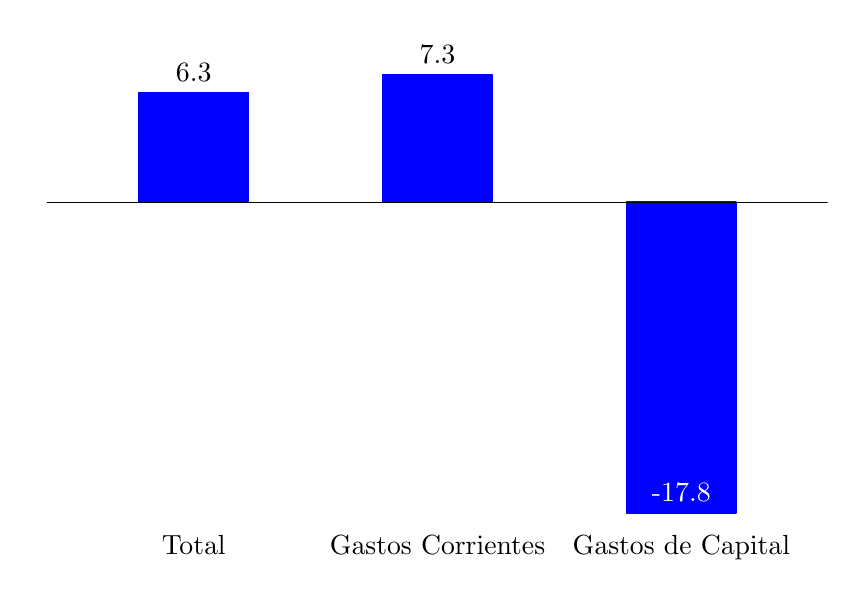
\begin{tikzpicture}[x=1pt,y=1pt]  % Created by tikzDevice version 0.7.0 on 2015-09-08 19:17:12
% !TEX encoding = UTF-8 Unicode
\definecolor[named]{fillColor}{rgb}{1.00,1.00,1.00}
\path[use as bounding box,fill=fillColor,fill opacity=0.00] (0,0) rectangle (289.08,198.74);
\begin{scope}
\path[clip] (  0.00,  0.00) rectangle (289.08,198.74);
\definecolor[named]{drawColor}{rgb}{1.00,1.00,1.00}

\path[draw=drawColor,line width= 0.6pt,line join=round,line cap=round] (  0.00,  0.00) rectangle (289.08,198.74);
\end{scope}
\begin{scope}
\path[clip] (  0.00,  0.00) rectangle (289.08,198.74);

\path[] (  7.11, 23.47) rectangle (289.08,181.67);

\path[] ( 59.98, 23.47) --
	( 59.98,181.67);

\path[] (148.10, 23.47) --
	(148.10,181.67);

\path[] (236.21, 23.47) --
	(236.21,181.67);
\definecolor[named]{drawColor}{rgb}{0.00,0.00,1.00}
\definecolor[named]{fillColor}{rgb}{0.00,0.00,1.00}

\path[draw=drawColor,line width= 0.6pt,line join=round,fill=fillColor] ( 40.16,135.66) rectangle ( 79.81,175.37);

\path[draw=drawColor,line width= 0.6pt,line join=round,fill=fillColor] (128.27,135.66) rectangle (167.92,181.67);

\path[draw=drawColor,line width= 0.6pt,line join=round,fill=fillColor] (216.39, 23.47) rectangle (256.04,135.66);
\definecolor[named]{drawColor}{rgb}{0.00,0.00,0.00}
\definecolor[named]{fillColor}{rgb}{0.00,0.00,0.00}

\path[draw=drawColor,line width= 0.1pt,line join=round,fill=fillColor] (  7.11,135.66) -- (289.08,135.66);

\node[text=drawColor,anchor=base,inner sep=0pt, outer sep=0pt, scale=  1.01] at ( 59.98,179.32) {6.3};

\node[text=drawColor,anchor=base,inner sep=0pt, outer sep=0pt, scale=  1.01] at (148.10,185.63) {7.3};

\node[text=white,anchor=base,inner sep=0pt, outer sep=0pt, scale=  1.01] at (236.21, 27.42) {-17.8};
\end{scope}
\begin{scope}
\path[clip] (  0.00,  0.00) rectangle (289.08,198.74);

\path[] (  7.11, 23.47) --
	(  7.11,181.67);
\end{scope}
\begin{scope}
\path[clip] (  0.00,  0.00) rectangle (289.08,198.74);

\path[] (  7.11, 23.47) --
	(289.08, 23.47);
\end{scope}
\begin{scope}
\path[clip] (  0.00,  0.00) rectangle (289.08,198.74);

\path[] ( 59.98, 19.20) --
	( 59.98, 23.47);

\path[] (148.10, 19.20) --
	(148.10, 23.47);

\path[] (236.21, 19.20) --
	(236.21, 23.47);
\end{scope}
\begin{scope}
\path[clip] (  0.00,  0.00) rectangle (289.08,198.74);
\definecolor[named]{drawColor}{rgb}{0.00,0.00,0.00}

\node[text=drawColor,anchor=base,inner sep=0pt, outer sep=0pt, scale=  1.00] at ( 59.98,  8.54) {Total};

\node[text=drawColor,anchor=base,inner sep=0pt, outer sep=0pt, scale=  1.00] at (148.10,  8.54) {Gastos Corrientes};

\node[text=drawColor,anchor=base,inner sep=0pt, outer sep=0pt, scale=  1.00] at (236.21,  8.54) {Gastos de Capital};
\end{scope}
  \end{tikzpicture}}{Instituto Nacional de Estadística}


\cajita{Evolución del gasto en educación por función}{Según la función en la que fue invertido el presupuesto,  el sector más impactado fue la educación preprimaria y primaria, que  representó el 53\% del presupuesto total y tuvo un crecimiento del 4.3\%. La educación media, tuvo una asignación del 12\% y un crecimiento del 4.7\%.  Asimismo, la educación superior tuvo un 13\% y un decrecimiento del 5.2\%.}{Gasto público en educación por función}{República de Guatemala, 2012 y 2013, en millones de quetzales de cada año	}{
	\ra{1.2}$\ $\\
	\begin{tabular}{p{7.5cm}rr}\hline
		\rowcolor{color2!15!white} &&\\[-4mm]
		{\Bold   Función         }&      \textbf{ 2012}   &  \textbf{ 2013   } \\
		\hline
		\rowcolor{white} &&\\[-4mm]
		
\textbf{Total}&	\textbf{12,133}& 	\textbf{12,896 }\\
Educación preprimaria y primaria&	6,609 &	6,894 \\
Servicios auxiliares de la educación&	1,273& 	1,725 \\
Educación universitaria o superior	&1,721 &	1,632 \\
Educación media	& 1,436 &	1,504 \\
Educación n.c.d &	624 &	662 \\
Educación no atribuible a ningún nivel escolarizado &	420 &	445 \\
Investigación y desarrollo relacionados con la educación&	23& 	25 \\
Educación postmedia básica y diversificado no universitaria&	27 &	9 \\

		\hline
		\rowcolor{white} &&\\[-5.5mm]
	
		&&\\[-0.09cm]
	\end{tabular}}{Instituto Nacional de Estadística}


\cajita{Gasto en educación por función}{La función con mayor incidencia  en relación a la asignación de gasto, ha sido la educación preprimaria y primaria, que representa el 53.5\% del total del gasto público en educación. El que tuvo la menor incidencia fue  el gasto en educación postmedia básica y diversificada, con el 0.1\% del gasto total.}{Distribución del gasto público en educación, por función}{República de Guatemala, 2013, en porcentaje}{\ \\[0mm]\begin{tikzpicture}[x=1pt,y=1pt]  % Created by tikzDevice version 0.7.0 on 2015-08-31 18:26:28
% !TEX encoding = UTF-8 Unicode
\definecolor[named]{fillColor}{rgb}{1.00,1.00,1.00}
\path[use as bounding box,fill=fillColor,fill opacity=0.00] (0,0) rectangle (289.08,198.74);
\begin{scope}
\path[clip] (  0.00,  0.00) rectangle (289.08,198.74);
\definecolor[named]{drawColor}{rgb}{1.00,1.00,1.00}

\path[draw=drawColor,line width= 0.6pt,line join=round,line cap=round] (  0.00,  0.00) rectangle (289.08,198.74);
\end{scope}
\begin{scope}
\path[clip] (  0.00,  0.00) rectangle (289.08,198.74);

\path[] ( -2.73, 17.78) rectangle (280.54,191.48);

\path[] (  0.00, 53.87) --
	(280.54, 53.87);

\path[] (  0.00,110.27) --
	(280.54,110.27);

\path[] (  0.00,166.67) --
	(280.54,166.67);

\path[] (  0.00, 25.67) --
	(280.54, 25.67);

\path[] (  0.00, 82.07) --
	(280.54, 82.07);

\path[] (  0.00,138.47) --
	(280.54,138.47);

\path[] ( 29.95, 17.78) --
	( 29.95,191.48);

\path[] ( 84.43, 17.78) --
	( 84.43,191.48);

\path[] (138.90, 17.78) --
	(138.90,191.48);

\path[] (193.38, 17.78) --
	(193.38,191.48);

\path[] (247.86, 17.78) --
	(247.86,191.48);
\definecolor[named]{drawColor}{rgb}{0.00,0.00,1.00}

\path[draw=drawColor,line width= 1.7pt,line join=round] ( 29.95,113.09) --
	( 84.43,110.27) --
	(138.90,104.63) --
	(193.38,183.59) --
	(247.86,152.57);
\definecolor[named]{drawColor}{rgb}{0.00,0.00,0.00}

\node[text=drawColor,anchor=base,inner sep=0pt, outer sep=0pt, scale=  1.01] at ( 29.95,117.05) {3.1};

\node[text=drawColor,anchor=base west,inner sep=0pt, outer sep=0pt, scale=  1.01] at ( 84.43,114.23) {3.0};

\node[text=drawColor,anchor=base,inner sep=0pt, outer sep=0pt, scale=  1.01] at (138.90, 92.76) {2.8};

\node[text=drawColor,anchor=base,inner sep=0pt, outer sep=0pt, scale=  1.01] at (193.38,187.54) {5.6};

\node[text=drawColor,anchor=base,inner sep=0pt, outer sep=0pt, scale=  1.01] at (247.86,140.70) {4.5};
\definecolor[named]{fillColor}{rgb}{0.00,0.00,0.00}

\path[draw=drawColor,line width= 0.1pt,line join=round,fill=fillColor] (  0.00, 25.67) -- (280.54, 25.67);
\end{scope}
\begin{scope}
\path[clip] (  0.00,  0.00) rectangle (289.08,198.74);

\path[] (  0.00, 17.78) --
	(280.54, 17.78);
\end{scope}
\begin{scope}
\path[clip] (  0.00,  0.00) rectangle (289.08,198.74);

\path[] ( 29.95, 13.51) --
	( 29.95, 17.78);

\path[] ( 84.43, 13.51) --
	( 84.43, 17.78);

\path[] (138.90, 13.51) --
	(138.90, 17.78);

\path[] (193.38, 13.51) --
	(193.38, 17.78);

\path[] (247.86, 13.51) --
	(247.86, 17.78);
\end{scope}
\begin{scope}
\path[clip] (  0.00,  0.00) rectangle (289.08,198.74);
\definecolor[named]{drawColor}{rgb}{0.00,0.00,0.00}

\node[text=drawColor,anchor=base,inner sep=0pt, outer sep=0pt, scale=  1.00] at ( 29.95,  2.85) {2009};

\node[text=drawColor,anchor=base,inner sep=0pt, outer sep=0pt, scale=  1.00] at ( 84.43,  2.85) {2010};

\node[text=drawColor,anchor=base,inner sep=0pt, outer sep=0pt, scale=  1.00] at (138.90,  2.85) {2011};

\node[text=drawColor,anchor=base,inner sep=0pt, outer sep=0pt, scale=  1.00] at (193.38,  2.85) {2012};

\node[text=drawColor,anchor=base,inner sep=0pt, outer sep=0pt, scale=  1.00] at (247.86,  2.85) {2013};
\end{scope}
  \end{tikzpicture}}{Instituto Nacional de Estadística}


\cajita{Crecimiento del gasto en educación por función}{
	La función que tuvo el mayor crecimiento de gasto, respecto al 2012, fueron los servicios auxiliares de educación, con el 35.5\%, seguido de la investigación y desarrollo en educación con el 9.5\%. \\
	
	El rubro con el mayor decrecimiento en la asignación de gasto fue la educación postmedia básica y diversificado, con el 68.1\% y la educación universitaria con el 5.2\%, respecto al año anterior.
	}{Tasa de crecimiento anual del gasto público en educación por función}{República de Guatemala, 2013, en porcentaje}{\ \\[0mm]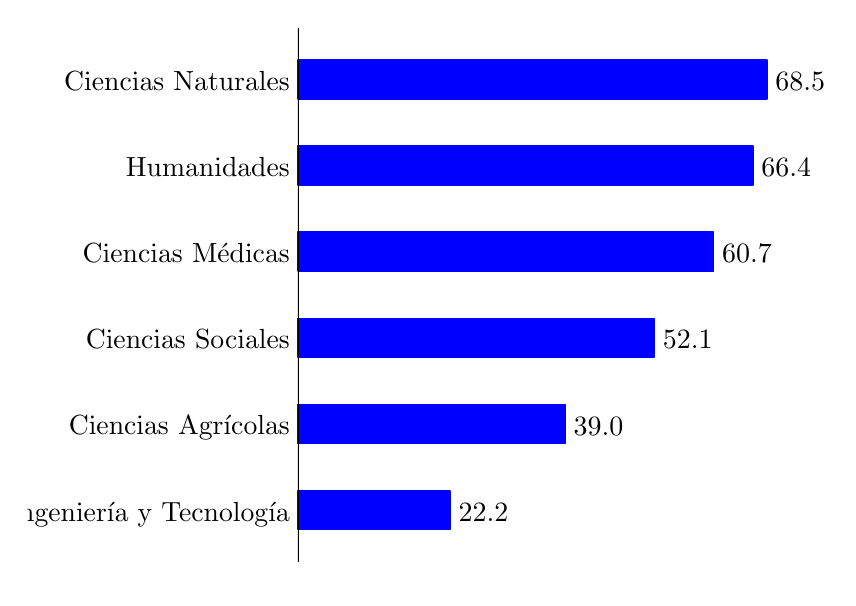
\begin{tikzpicture}[x=1pt,y=1pt]  % Created by tikzDevice version 0.7.0 on 2015-08-31 14:52:10
% !TEX encoding = UTF-8 Unicode
\definecolor[named]{fillColor}{rgb}{1.00,1.00,1.00}
\path[use as bounding box,fill=fillColor,fill opacity=0.00] (0,0) rectangle (289.08,198.74);
\begin{scope}
\path[clip] (  0.00,  0.00) rectangle (289.08,198.74);
\definecolor[named]{drawColor}{rgb}{1.00,1.00,1.00}

\path[draw=drawColor,line width= 0.6pt,line join=round,line cap=round] (  0.00,  0.00) rectangle (289.08,198.74);
\end{scope}
\begin{scope}
\path[clip] (  0.00,  0.00) rectangle (289.08,198.74);

\path[] ( 97.57,  5.69) rectangle (267.09,198.74);

\path[] ( 97.57, 24.37) --
	(267.09, 24.37);

\path[] ( 97.57, 55.51) --
	(267.09, 55.51);

\path[] ( 97.57, 86.65) --
	(267.09, 86.65);

\path[] ( 97.57,117.79) --
	(267.09,117.79);

\path[] ( 97.57,148.92) --
	(267.09,148.92);

\path[] ( 97.57,180.06) --
	(267.09,180.06);
\definecolor[named]{drawColor}{rgb}{0.00,0.00,1.00}
\definecolor[named]{fillColor}{rgb}{0.00,0.00,1.00}

\path[draw=drawColor,line width= 0.6pt,line join=round,fill=fillColor] ( 97.57, 17.37) rectangle (152.65, 31.38);

\path[draw=drawColor,line width= 0.6pt,line join=round,fill=fillColor] ( 97.57, 48.50) rectangle (194.18, 62.52);

\path[draw=drawColor,line width= 0.6pt,line join=round,fill=fillColor] ( 97.57, 79.64) rectangle (226.45, 93.65);

\path[draw=drawColor,line width= 0.6pt,line join=round,fill=fillColor] ( 97.57,110.78) rectangle (247.82,124.79);

\path[draw=drawColor,line width= 0.6pt,line join=round,fill=fillColor] ( 97.57,141.92) rectangle (262.01,155.93);

\path[draw=drawColor,line width= 0.6pt,line join=round,fill=fillColor] ( 97.57,173.05) rectangle (267.09,187.07);
\definecolor[named]{drawColor}{rgb}{0.00,0.00,0.00}
\definecolor[named]{fillColor}{rgb}{0.00,0.00,0.00}

\path[draw=drawColor,line width= 0.1pt,line join=round,fill=fillColor] ( 97.57,  5.69) -- ( 97.57,198.74);

\node[text=drawColor,anchor=base west,inner sep=0pt, outer sep=0pt, scale=  1.01] at (155.76, 20.42) {22.2};

\node[text=drawColor,anchor=base west,inner sep=0pt, outer sep=0pt, scale=  1.01] at (197.29, 51.55) {39.0};

\node[text=drawColor,anchor=base west,inner sep=0pt, outer sep=0pt, scale=  1.01] at (229.57, 82.69) {52.1};

\node[text=drawColor,anchor=base west,inner sep=0pt, outer sep=0pt, scale=  1.01] at (250.94,113.83) {60.7};

\node[text=drawColor,anchor=base west,inner sep=0pt, outer sep=0pt, scale=  1.01] at (265.12,144.97) {66.4};

\node[text=drawColor,anchor=base west,inner sep=0pt, outer sep=0pt, scale=  1.01] at (270.20,176.10) {68.5};
\end{scope}
\begin{scope}
\path[clip] (  0.00,  0.00) rectangle (289.08,198.74);

\path[] ( 97.57,  5.69) --
	( 97.57,198.74);
\end{scope}
\begin{scope}
\path[clip] (  0.00,  0.00) rectangle (289.08,198.74);
\definecolor[named]{drawColor}{rgb}{0.00,0.00,0.00}

\node[text=drawColor,anchor=base east,inner sep=0pt, outer sep=0pt, scale=  1.00] at ( 94.72, 20.46) {Ingenier\'ia y Tecnolog\'ia};

\node[text=drawColor,anchor=base east,inner sep=0pt, outer sep=0pt, scale=  1.00] at ( 94.72, 51.60) {Ciencias Agr\'icolas};

\node[text=drawColor,anchor=base east,inner sep=0pt, outer sep=0pt, scale=  1.00] at ( 94.72, 82.74) {Ciencias Sociales};

\node[text=drawColor,anchor=base east,inner sep=0pt, outer sep=0pt, scale=  1.00] at ( 94.72,113.88) {Ciencias M\'edicas};

\node[text=drawColor,anchor=base east,inner sep=0pt, outer sep=0pt, scale=  1.00] at ( 94.72,145.01) {Humanidades};

\node[text=drawColor,anchor=base east,inner sep=0pt, outer sep=0pt, scale=  1.00] at ( 94.72,176.15) {Ciencias Naturales };
\end{scope}
\begin{scope}
\path[clip] (  0.00,  0.00) rectangle (289.08,198.74);

\path[] ( 94.72, 24.37) --
	( 98.99, 24.37);

\path[] ( 94.72, 55.51) --
	( 98.99, 55.51);

\path[] ( 94.72, 86.65) --
	( 98.99, 86.65);

\path[] ( 94.72,117.79) --
	( 98.99,117.79);

\path[] ( 94.72,148.92) --
	( 98.99,148.92);

\path[] ( 94.72,180.06) --
	( 98.99,180.06);
\end{scope}
\begin{scope}
\path[clip] (  0.00,  0.00) rectangle (289.08,198.74);

\path[] ( 97.57,  5.69) --
	(267.09,  5.69);
\end{scope}
  \end{tikzpicture}}{Instituto Nacional de Estadística}


\cajita{Evolución de las fuentes de financiamiento}{De acuerdo a la fuente de financiamiento, la mas importante provino de recursos del tesoro (con y sin afectación específica) de donde se obtuvo el 95\% del presupuesto y este tuvo aumento del 13\% respecto del año anterior. El 0.26\% del gasto público en educación provino de donaciones externas.}{Gasto público en educación por fuente de financiamiento agregada}{República de Guatemala, 2012 y 2013, en millones de quetzales de cada año}{
	\ra{1.2}$\ $\\
	\begin{tabular}{p{6cm}rr}\hline
		\rowcolor{color2!15!white} &&\\[-4mm]
		{\Bold   Fuente de financiamiento         }&      \textbf{ 2012}   &  \textbf{ 2013 }   \\
		\hline
		\rowcolor{white} &&\\[-4mm]
		
	\textbf{	Total}&	\textbf{12,133}& 	\textbf{12,896}  \\
	Recursos del Tesoro&	7,625 &	8,912  \\
		Recursos del Tesoro con Afectación Especifica&	3,194 &	3,342  \\
		Recursos Propios de las Instituciones&	387 & 378  \\
		Crédito Externo&	877 &	231  \\
		Donaciones Externas&	50 	& 33  \\
		
		\hline
		\rowcolor{white} &&\\[-5.5mm]

		&&\\[-0.09cm]
	\end{tabular}}{Instituto Nacional de Estadística}


\cajita{Fuentes de financiamiento}{La fuente de financiamiento con mayor incidencia  en relación a la asignación obtenida, fueron los recursos del tesoro, que representó el 69.1\% del total del gasto público en educación. El que tuvo la menor incidencia fueron las donaciones externas, con el  0.3\% del financiamiento en gasto público en educación total.}{Distribución del gasto público en educación por fuente de financiamiento agregada}{República de Guatemala, 2013, en porcentaje}{\ \\[0mm]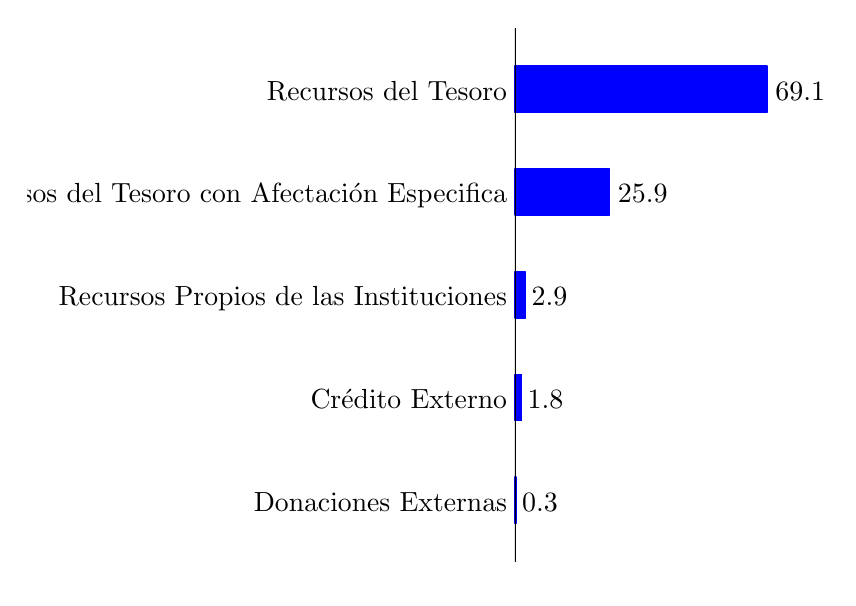
\begin{tikzpicture}[x=1pt,y=1pt]  % Created by tikzDevice version 0.7.0 on 2015-08-28 16:35:08
% !TEX encoding = UTF-8 Unicode
\definecolor[named]{fillColor}{rgb}{1.00,1.00,1.00}
\path[use as bounding box,fill=fillColor,fill opacity=0.00] (0,0) rectangle (289.08,198.74);
\begin{scope}
\path[clip] (  0.00,  0.00) rectangle (289.08,198.74);
\definecolor[named]{drawColor}{rgb}{1.00,1.00,1.00}

\path[draw=drawColor,line width= 0.6pt,line join=round,line cap=round] (  0.00,  0.00) rectangle (289.08,198.74);
\end{scope}
\begin{scope}
\path[clip] (  0.00,  0.00) rectangle (289.08,198.74);

\path[] (176.08,  5.69) rectangle (267.09,198.74);

\path[] (176.08, 27.97) --
	(267.09, 27.97);

\path[] (176.08, 65.09) --
	(267.09, 65.09);

\path[] (176.08,102.22) --
	(267.09,102.22);

\path[] (176.08,139.34) --
	(267.09,139.34);

\path[] (176.08,176.47) --
	(267.09,176.47);
\definecolor[named]{drawColor}{rgb}{0.00,0.00,1.00}
\definecolor[named]{fillColor}{rgb}{0.00,0.00,1.00}

\path[draw=drawColor,line width= 0.6pt,line join=round,fill=fillColor] (176.08, 19.61) rectangle (176.47, 36.32);

\path[draw=drawColor,line width= 0.6pt,line join=round,fill=fillColor] (176.08, 56.74) rectangle (178.45, 73.44);

\path[draw=drawColor,line width= 0.6pt,line join=round,fill=fillColor] (176.08, 93.86) rectangle (179.90,110.57);

\path[draw=drawColor,line width= 0.6pt,line join=round,fill=fillColor] (176.08,130.99) rectangle (210.19,147.70);

\path[draw=drawColor,line width= 0.6pt,line join=round,fill=fillColor] (176.08,168.11) rectangle (267.09,184.82);
\definecolor[named]{drawColor}{rgb}{0.00,0.00,0.00}
\definecolor[named]{fillColor}{rgb}{0.00,0.00,0.00}

\path[draw=drawColor,line width= 0.1pt,line join=round,fill=fillColor] (176.08,  5.69) -- (176.08,198.74);

\node[text=drawColor,anchor=base west,inner sep=0pt, outer sep=0pt, scale=  1.01] at (178.70, 24.01) {0.3};

\node[text=drawColor,anchor=base west,inner sep=0pt, outer sep=0pt, scale=  1.01] at (180.68, 61.13) {1.8};

\node[text=drawColor,anchor=base west,inner sep=0pt, outer sep=0pt, scale=  1.01] at (182.13, 98.26) {2.9};

\node[text=drawColor,anchor=base west,inner sep=0pt, outer sep=0pt, scale=  1.01] at (213.30,135.39) {25.9};

\node[text=drawColor,anchor=base west,inner sep=0pt, outer sep=0pt, scale=  1.01] at (270.20,172.51) {69.1};
\end{scope}
\begin{scope}
\path[clip] (  0.00,  0.00) rectangle (289.08,198.74);

\path[] (176.08,  5.69) --
	(176.08,198.74);
\end{scope}
\begin{scope}
\path[clip] (  0.00,  0.00) rectangle (289.08,198.74);
\definecolor[named]{drawColor}{rgb}{0.00,0.00,0.00}

\node[text=drawColor,anchor=base east,inner sep=0pt, outer sep=0pt, scale=  1.00] at (173.23, 24.06) {Donaciones Externas};

\node[text=drawColor,anchor=base east,inner sep=0pt, outer sep=0pt, scale=  1.00] at (173.23, 61.18) {Cr\'edito Externo};

\node[text=drawColor,anchor=base east,inner sep=0pt, outer sep=0pt, scale=  1.00] at (173.23, 98.31) {Recursos Propios de las Instituciones};

\node[text=drawColor,anchor=base east,inner sep=0pt, outer sep=0pt, scale=  1.00] at (173.23,135.43) {Recursos del Tesoro con Afectaci\'on Especifica};

\node[text=drawColor,anchor=base east,inner sep=0pt, outer sep=0pt, scale=  1.00] at (173.23,172.56) {Recursos del Tesoro};
\end{scope}
\begin{scope}
\path[clip] (  0.00,  0.00) rectangle (289.08,198.74);

\path[] (173.23, 27.97) --
	(177.50, 27.97);

\path[] (173.23, 65.09) --
	(177.50, 65.09);

\path[] (173.23,102.22) --
	(177.50,102.22);

\path[] (173.23,139.34) --
	(177.50,139.34);

\path[] (173.23,176.47) --
	(177.50,176.47);
\end{scope}
\begin{scope}
\path[clip] (  0.00,  0.00) rectangle (289.08,198.74);

\path[] (176.08,  5.69) --
	(267.09,  5.69);
\end{scope}
  \end{tikzpicture}}{Instituto Nacional de Estadística}


\cajita{Crecimiento de la fuentes de financiamiento}{La fuente de financiamiento que tuvo el mayor crecimiento de asignación, respecto al 2012, fueron los recursos del tesoro, con el 16.9\%, seguido de los recursos del tesoro con afectación específica, con el 4.6\%.\\
	
	 El rubro con el mayor decrecimiento en el financiamiento del gasto público en educación  fue el crédito externo, con el 73.6\% y las donaciones externas, con el 34.6\%, respecto al año anterior.}{Tasa de crecimiento anual del gasto público en educación por fuente de financiamiento agregada}{República de Guatemala, 2013, en porcentaje}{\ \\[0mm]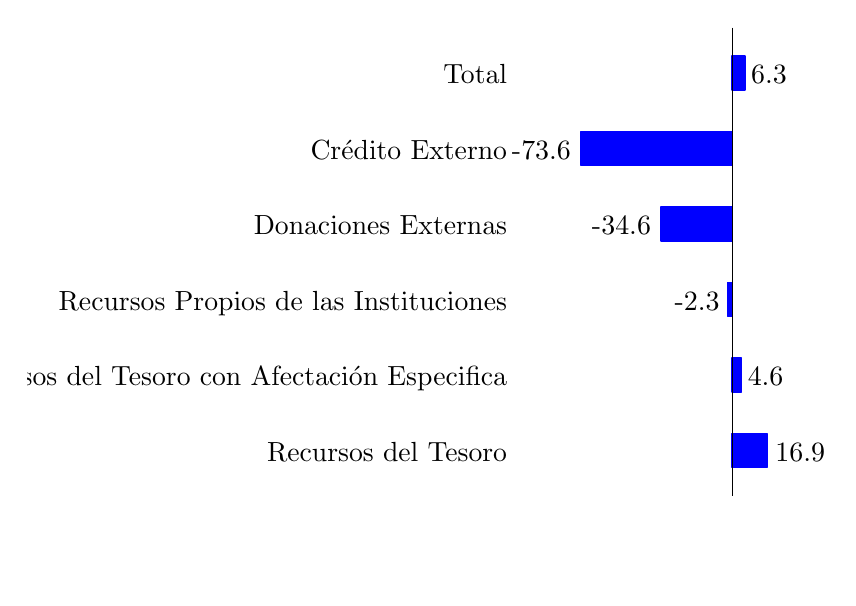
\begin{tikzpicture}[x=1pt,y=1pt]  % Created by tikzDevice version 0.7.0 on 2015-08-28 16:35:09
% !TEX encoding = UTF-8 Unicode
\definecolor[named]{fillColor}{rgb}{1.00,1.00,1.00}
\path[use as bounding box,fill=fillColor,fill opacity=0.00] (0,0) rectangle (289.08,198.74);
\begin{scope}
\path[clip] (  0.00,  0.00) rectangle (289.08,198.74);
\definecolor[named]{drawColor}{rgb}{1.00,1.00,1.00}

\path[draw=drawColor,line width= 0.6pt,line join=round,line cap=round] (  0.00,  0.00) rectangle (289.08,198.74);
\end{scope}
\begin{scope}
\path[clip] (  0.00,  0.00) rectangle (289.08,198.74);

\path[] (199.99, 29.60) rectangle (267.09,198.74);

\path[] (199.99, 45.97) --
	(267.09, 45.97);

\path[] (199.99, 73.25) --
	(267.09, 73.25);

\path[] (199.99,100.53) --
	(267.09,100.53);

\path[] (199.99,127.81) --
	(267.09,127.81);

\path[] (199.99,155.09) --
	(267.09,155.09);

\path[] (199.99,182.37) --
	(267.09,182.37);
\definecolor[named]{drawColor}{rgb}{0.00,0.00,1.00}
\definecolor[named]{fillColor}{rgb}{0.00,0.00,1.00}

\path[draw=drawColor,line width= 0.6pt,line join=round,fill=fillColor] (254.56, 39.83) rectangle (267.09, 52.11);

\path[draw=drawColor,line width= 0.6pt,line join=round,fill=fillColor] (254.56, 67.11) rectangle (257.97, 79.39);

\path[draw=drawColor,line width= 0.6pt,line join=round,fill=fillColor] (252.85, 94.39) rectangle (254.56,106.67);

\path[draw=drawColor,line width= 0.6pt,line join=round,fill=fillColor] (228.90,121.67) rectangle (254.56,133.95);

\path[draw=drawColor,line width= 0.6pt,line join=round,fill=fillColor] (199.99,148.95) rectangle (254.56,161.23);

\path[draw=drawColor,line width= 0.6pt,line join=round,fill=fillColor] (254.56,176.24) rectangle (259.23,188.51);
\definecolor[named]{drawColor}{rgb}{0.00,0.00,0.00}
\definecolor[named]{fillColor}{rgb}{0.00,0.00,0.00}

\path[draw=drawColor,line width= 0.1pt,line join=round,fill=fillColor] (254.56, 29.60) -- (254.56,198.74);

\node[text=drawColor,anchor=base west,inner sep=0pt, outer sep=0pt, scale=  1.01] at (270.20, 42.01) {16.9};

\node[text=drawColor,anchor=base west,inner sep=0pt, outer sep=0pt, scale=  1.01] at (260.20, 69.29) {4.6};

\node[text=drawColor,anchor=base east,inner sep=0pt, outer sep=0pt, scale=  1.01] at (250.06, 96.57) {-2.3};

\node[text=drawColor,anchor=base east,inner sep=0pt, outer sep=0pt, scale=  1.01] at (225.23,123.86) {-34.6};

\node[text=drawColor,anchor=base east,inner sep=0pt, outer sep=0pt, scale=  1.01] at (196.31,151.14) {-73.6};

\node[text=drawColor,anchor=base west,inner sep=0pt, outer sep=0pt, scale=  1.01] at (261.46,178.42) {6.3};
\end{scope}
\begin{scope}
\path[clip] (  0.00,  0.00) rectangle (289.08,198.74);

\path[] (199.99, 29.60) --
	(199.99,198.74);
\end{scope}
\begin{scope}
\path[clip] (  0.00,  0.00) rectangle (289.08,198.74);
\definecolor[named]{drawColor}{rgb}{0.00,0.00,0.00}

\node[text=drawColor,anchor=base east,inner sep=0pt, outer sep=0pt, scale=  1.00] at (173.23, 42.06) {Recursos del Tesoro};

\node[text=drawColor,anchor=base east,inner sep=0pt, outer sep=0pt, scale=  1.00] at (173.23, 69.34) {Recursos del Tesoro con Afectaci\'on Especifica};

\node[text=drawColor,anchor=base east,inner sep=0pt, outer sep=0pt, scale=  1.00] at (173.23, 96.62) {Recursos Propios de las Instituciones};

\node[text=drawColor,anchor=base east,inner sep=0pt, outer sep=0pt, scale=  1.00] at (173.23,123.90) {Donaciones Externas};

\node[text=drawColor,anchor=base east,inner sep=0pt, outer sep=0pt, scale=  1.00] at (173.23,151.18) {Cr\'edito Externo};

\node[text=drawColor,anchor=base east,inner sep=0pt, outer sep=0pt, scale=  1.00] at (173.23,178.47) {Total};
\end{scope}
\begin{scope}
\path[clip] (  0.00,  0.00) rectangle (289.08,198.74);

\path[] (173.23, 45.97) --
	(177.50, 45.97);

\path[] (173.23, 73.25) --
	(177.50, 73.25);

\path[] (173.23,100.53) --
	(177.50,100.53);

\path[] (173.23,127.81) --
	(177.50,127.81);

\path[] (173.23,155.09) --
	(177.50,155.09);

\path[] (173.23,182.37) --
	(177.50,182.37);
\end{scope}
\begin{scope}
\path[clip] (  0.00,  0.00) rectangle (289.08,198.74);

\path[] (199.99, 29.60) --
	(267.09, 29.60);
\end{scope}
  \end{tikzpicture}}{Instituto Nacional de Estadística}


\cajita{Gasto en educación en relación al PIB}{El gasto público en educación como porcentaje del producto interno bruto tuvo una variación de 0.1 puntos porcentuales, respecto del 2012.
	Asimismo, en el 2013 de la totalidad del gasto público, el 21.3\% fue asignado para educación, teniendo un aumento de 0.3 puntos porcentuales respecto al 2012.
	}{Gasto público en educación como porcentaje del producto interno bruto y el gasto público}{República de Guatemala, 2012 y 2013, en porcentaje}{\ \\[0mm]\begin{tikzpicture}[x=1pt,y=1pt]  % Created by tikzDevice version 0.7.0 on 2015-08-31 18:35:32
% !TEX encoding = UTF-8 Unicode
\definecolor[named]{fillColor}{rgb}{1.00,1.00,1.00}
\path[use as bounding box,fill=fillColor,fill opacity=0.00] (0,0) rectangle (289.08,198.74);
\begin{scope}
\path[clip] (  0.00,  0.00) rectangle (289.08,198.74);
\definecolor[named]{drawColor}{rgb}{1.00,1.00,1.00}

\path[draw=drawColor,line width= 0.6pt,line join=round,line cap=round] (  0.00,  0.00) rectangle (289.08,198.74);
\end{scope}
\begin{scope}
\path[clip] (  0.00,  0.00) rectangle (289.08,198.74);

\path[] (  1.64, 17.78) rectangle (280.54,191.48);

\path[] (  1.64, 48.89) --
	(280.54, 48.89);

\path[] (  1.64, 95.34) --
	(280.54, 95.34);

\path[] (  1.64,141.79) --
	(280.54,141.79);

\path[] (  1.64,188.23) --
	(280.54,188.23);

\path[] (  1.64, 25.67) --
	(280.54, 25.67);

\path[] (  1.64, 72.12) --
	(280.54, 72.12);

\path[] (  1.64,118.56) --
	(280.54,118.56);

\path[] (  1.64,165.01) --
	(280.54,165.01);

\path[] ( 33.83, 17.78) --
	( 33.83,191.48);

\path[] ( 87.46, 17.78) --
	( 87.46,191.48);

\path[] (141.09, 17.78) --
	(141.09,191.48);

\path[] (194.73, 17.78) --
	(194.73,191.48);

\path[] (248.36, 17.78) --
	(248.36,191.48);
\definecolor[named]{drawColor}{rgb}{0.00,0.00,1.00}

\path[draw=drawColor,line width= 1.7pt,line join=round] ( 33.83,132.50) --
	( 87.46,183.59) --
	(141.09,114.85) --
	(194.73,103.70) --
	(248.36, 89.77);
\definecolor[named]{drawColor}{rgb}{0.00,0.00,0.00}

\node[text=drawColor,anchor=base,inner sep=0pt, outer sep=0pt, scale=  1.01] at ( 33.83,120.63) {6.5};

\node[text=drawColor,anchor=base,inner sep=0pt, outer sep=0pt, scale=  1.01] at ( 87.46,187.54) {12.0};

\node[text=drawColor,anchor=base west,inner sep=0pt, outer sep=0pt, scale=  1.01] at (141.09,118.80) {4.6};

\node[text=drawColor,anchor=base west,inner sep=0pt, outer sep=0pt, scale=  1.01] at (194.73,107.66) {3.4};

\node[text=drawColor,anchor=base,inner sep=0pt, outer sep=0pt, scale=  1.01] at (248.36, 77.90) {1.9};
\definecolor[named]{fillColor}{rgb}{0.00,0.00,0.00}

\path[draw=drawColor,line width= 0.1pt,line join=round,fill=fillColor] (  1.64, 25.67) -- (280.54, 25.67);
\end{scope}
\begin{scope}
\path[clip] (  0.00,  0.00) rectangle (289.08,198.74);

\path[] (  1.64, 17.78) --
	(  1.64,191.48);
\end{scope}
\begin{scope}
\path[clip] (  0.00,  0.00) rectangle (289.08,198.74);

\path[] (  0.00, 25.67) --
	(  1.64, 25.67);

\path[] (  0.00, 72.12) --
	(  1.64, 72.12);

\path[] (  0.00,118.56) --
	(  1.64,118.56);

\path[] (  0.00,165.01) --
	(  1.64,165.01);
\end{scope}
\begin{scope}
\path[clip] (  0.00,  0.00) rectangle (289.08,198.74);

\path[] (  1.64, 17.78) --
	(280.54, 17.78);
\end{scope}
\begin{scope}
\path[clip] (  0.00,  0.00) rectangle (289.08,198.74);

\path[] ( 33.83, 13.51) --
	( 33.83, 17.78);

\path[] ( 87.46, 13.51) --
	( 87.46, 17.78);

\path[] (141.09, 13.51) --
	(141.09, 17.78);

\path[] (194.73, 13.51) --
	(194.73, 17.78);

\path[] (248.36, 13.51) --
	(248.36, 17.78);
\end{scope}
\begin{scope}
\path[clip] (  0.00,  0.00) rectangle (289.08,198.74);
\definecolor[named]{drawColor}{rgb}{0.00,0.00,0.00}

\node[text=drawColor,anchor=base,inner sep=0pt, outer sep=0pt, scale=  1.00] at ( 33.83,  2.85) {2009};

\node[text=drawColor,anchor=base,inner sep=0pt, outer sep=0pt, scale=  1.00] at ( 87.46,  2.85) {2010};

\node[text=drawColor,anchor=base,inner sep=0pt, outer sep=0pt, scale=  1.00] at (141.09,  2.85) {2011};

\node[text=drawColor,anchor=base,inner sep=0pt, outer sep=0pt, scale=  1.00] at (194.73,  2.85) {2012};

\node[text=drawColor,anchor=base,inner sep=0pt, outer sep=0pt, scale=  1.00] at (248.36,  2.85) {2013};
\end{scope}
  \end{tikzpicture}}{Instituto Nacional de Estadística}
